\documentclass[12pt,a4paper,oneside]{report}
\usepackage[utf8]{inputenc}
\usepackage[T1]{fontenc}
\usepackage[french]{babel}
\usepackage{lmodern}
\usepackage{microtype}
\usepackage{geometry}
\geometry{top=2.4cm,bottom=2.4cm,left=2.7cm,right=2.4cm}
\usepackage{graphicx}
\usepackage{booktabs,longtable,tabularx,array,multirow}
\usepackage[table]{xcolor}
\usepackage{enumitem}
\usepackage{listings}
\usepackage{tikz}
\usetikzlibrary{arrows.meta,positioning,shapes.geometric,fit,calc}
\usepackage{float}
\usepackage{caption}
\usepackage{subcaption}
\usepackage{fancyhdr}
\usepackage{lastpage}
\usepackage{hyperref}
\usepackage{url}

\definecolor{AuditGreen}{HTML}{0B7A63}
\definecolor{AuditNavy}{HTML}{10243E}
\definecolor{AuditLight}{HTML}{EEF5F3}
\definecolor{AuditGray}{HTML}{5E6B78}
\hypersetup{colorlinks=true,linkcolor=AuditNavy,urlcolor=AuditGreen,citecolor=AuditGreen,pdftitle={Rapport final AuditHub},pdfauthor={Auteur non communiqu\'e}}
\setlength{\parindent}{0pt}
\setlength{\parskip}{0.55em}
\setlength{\tabcolsep}{4pt}
\setlength{\emergencystretch}{2em}
\setlist{nosep,leftmargin=1.6em}
\captionsetup{font=small,labelfont=bf}
\renewcommand{\arraystretch}{1.22}
\pagestyle{fancy}
\fancyhf{}
\fancyhead[L]{\textcolor{AuditGray}{AuditHub --- Rapport final}}
\fancyhead[R]{\textcolor{AuditGray}{Projet Django + React}}
\fancyfoot[C]{\thepage\ / \pageref{LastPage}}
\setlength{\headheight}{15pt}
\lstset{basicstyle=\ttfamily\small,breaklines=true,frame=single,rulecolor=\color{AuditLight},backgroundcolor=\color{AuditLight},showstringspaces=false}
\newcommand{\evidence}[1]{\nolinkurl{#1}}
\newcommand{\nonverifie}{\textit{Information non communiqu\'ee ou non v\'erifiable dans le d\'ep\^ot.}}

\begin{document}
\pagenumbering{gobble}
\begin{titlepage}
  \pagecolor{AuditNavy}\color{white}
  \vspace*{1.2cm}
  {\Large\bfseries RAPPORT FINAL DE PROJET\par}
  \vspace{1.2cm}
  {\Huge\bfseries AuditHub\par}
  \vspace{0.4cm}
  {\LARGE Plateforme de gestion documentaire des audits techniques\par}
  \vfill
  \begin{tabular}{@{}ll@{}}
    \textbf{Nature :} & Projet acad\'emique d'ing\'enierie logicielle\\
    \textbf{Technologies :} & Django 5.2, React 19, SQLite, Playwright\\
    \textbf{Date du rapport :} & 15 octobre 2026\\
    \textbf{Version :} & 1.0\\
    \textbf{Classification :} & CONFIDENTIEL --- remise acad\'emique\\
    \textbf{Auteur / encadrant :} & Informations non communiqu\'ees\\
  \end{tabular}
  \vfill
  {\large Rapport fond\'e sur l'impl\'ementation effectivement pr\'esente dans le d\'ep\^ot.\par}
\end{titlepage}
\nopagecolor\color{black}

\pagenumbering{roman}
\chapter*{Avertissement sur la nature du document}
\addcontentsline{toc}{chapter}{Avertissement sur la nature du document}
Le document de r\'ef\'erence fourni adopte la structure d'un rapport d'audit de SMSI. Le pr\'esent livrable l'applique \`a l'\'evaluation technique du projet logiciel AuditHub. Il ne constitue ni un audit de certification ISO/IEC 27001, ni une recommandation de certification, ni une preuve de conformit\'e d'une organisation. Les informations institutionnelles, identit\'es, signatures et d\'ecisions qui ne figurent pas dans le d\'ep\^ot sont explicitement signal\'ees comme non v\'erifiables.

\tableofcontents
\listoffigures
\listoftables
\clearpage
\pagenumbering{arabic}

\chapter{INFORMATIONS G\'EN\'ERALES}

\section*{Pr\'esentation du projet}
\addcontentsline{toc}{section}{Pr\'esentation du projet}
AuditHub est une application web monoproduit destin\'ee \`a centraliser la documentation de missions de tests d'intrusion autoris\'es. Elle associe une interface React \`a une API JSON Django. Son r\^ole n'est pas d'ex\'ecuter Nmap, Metasploit, Burp Suite ou OWASP ZAP : les outils restent utilis\'es dans un laboratoire externe autoris\'e, puis leurs r\'esultats sont consign\'es sous forme textuelle dans l'application.

Le besoin trait\'e est la dispersion habituelle des informations d'un audit technique : autorisation, p\'erim\`etre IP, intervenants, m\'ethode, preuve, s\'ev\'erit\'e, responsable de correction, \`ech\'eance et re-test. AuditHub rassemble ces objets dans une cha\^ine tra\c{c}able et applique des contr\^oles d'acc\`es c\^ot\'e serveur.

\begin{table}[H]
\centering
\caption{Fiche d'identit\'e technique d'AuditHub}
\begin{tabularx}{\textwidth}{>{\bfseries}p{4.1cm}X}
\toprule
\rowcolor{AuditLight}Rubrique & Information v\'erifi\'ee\\
\midrule
Backend & Django 5.2.17, vues fonctionnelles, formulaires et ORM\\
Frontend & React 19.3.0, bundle ES2020 produit par esbuild 0.28.2\\
Persistance & SQLite, migration applicative jusqu'\`a \evidence{0002\_followup\_constraints}\\
Authentification & Sessions Django, cookie HttpOnly, jeton CSRF, limitation des \`echecs\\
R\^oles & Administrateur, Pentesteur, Auditeur\\
Tests & 33 tests Django et 3 parcours Playwright valid\'es le 15 octobre 2026\\
D\'eploiement document\'e & Waitress derri\`ere un reverse proxy TLS ; variables d'environnement obligatoires\\
\bottomrule
\end{tabularx}
\end{table}

\section*{1.3 Type d'audit}
\addcontentsline{toc}{section}{1.3 Type d'audit}
Le travail rapport\'e est une \textbf{revue technique et fonctionnelle du logiciel}, compl\'et\'ee par l'ex\'ecution de ses tests automatis\'es. Il ne s'agit pas d'un audit initial, de surveillance ou de renouvellement d'un SMSI au sens d'un organisme de certification. Cette qualification est essentielle : le d\'ep\^ot ne contient ni mandat de certification, ni D\'eclaration d'Applicabilit\'e organisationnelle, ni entretiens, ni preuves d'un environnement de production.

\section*{1.4 Dates et dur\'ee de l'audit}
\addcontentsline{toc}{section}{1.4 Dates et dur\'ee de l'audit}
L'\'etat final analys\'e et les validations pr\'esent\'ees dans ce rapport datent du \textbf{15 octobre 2026}. La date de cr\'eation du rapport de tests historique du projet est le 1\textsuperscript{er} octobre 2026, puis il a \`et\'e actualis\'e. La dur\'ee humaine totale de conception et de d\'eveloppement n'est pas enregistr\'ee dans le d\'ep\^ot ; elle ne peut donc pas \^etre chiffr\'ee sans supposition.

\section*{Probl\'ematique et besoins}
\addcontentsline{toc}{section}{Probl\'ematique et besoins}
La probl\'ematique peut \^etre formul\'ee ainsi : \emph{comment fournir une application simple, tra\c{c}able et contr\^ol\'ee pour documenter des tests de s\'ecurit\'e r\'ealis\'es hors plateforme, sans transformer le serveur web en outil offensif ?} La r\'eponse impl\'ement\'ee repose sur la s\'eparation entre ex\'ecution et documentation, un p\'erim\`etre explicite par mission, des r\^oles, la journalisation et un export JSON.

\chapter{OBJECTIFS DE L'AUDIT}

L'objectif de cette revue est d'\'evaluer si la version finale d'AuditHub correspond \`a son positionnement document\'e et si ses principaux m\'ecanismes sont coh\'erents avec le code, les migrations et les tests. Elle ne cherche pas \`a conclure sur l'efficacit\'e globale d'un SMSI r\'eel.

\section*{Objectifs fonctionnels}
\addcontentsline{toc}{section}{Objectifs fonctionnels}
\begin{itemize}
  \item v\'erifier la gestion de missions avec r\'ef\'erence d'autorisation, dates, p\'erim\`etre IP/CIDR et membres ;
  \item v\'erifier la saisie de constats issus de quatre familles d'outils, avec m\'ethode, preuve, s\'ev\'erit\'e et correction ;
  \item examiner le suivi dat\'e et l'historique des re-tests ;
  \item contr\^oler les exports de mission et du journal ;
  \item d\'ecrire les parcours React r\'eellement disponibles.
\end{itemize}

\section*{Objectifs de s\'ecurit\'e et de qualit\'e}
\addcontentsline{toc}{section}{Objectifs de s\'ecurit\'e et de qualit\'e}
La revue couvre l'authentification par session, les permissions fond\'ees sur trois r\^oles, le cloisonnement par mission, CSRF, l'\'echappement des preuves affich\'ees par React, les en-t\^etes HTTP, la limitation des tentatives de connexion, les contraintes de base et la gestion des secrets de configuration. Elle v\'erifie aussi la reproductibilit\'e du build et l'existence d'une cha\^ine d'int\'egration continue.

\section*{Crit\`eres de r\'eussite retenus}
\addcontentsline{toc}{section}{Crit\`eres de r\'eussite retenus}
Une exigence est consid\'er\'ee comme mise en \oe uvre seulement lorsqu'elle est observable dans le code, la migration, l'interface ou un test. La simple pr\'esence d'un texte dans la documentation ne suffit pas. Inversement, les fonctions explicitement hors p\'erim\`etre --- ex\'ecution de scanners, import de fichiers, MFA, SSO ou certification --- ne sont pas pr\'esent\'ees comme livr\'ees.

\begin{table}[H]
\centering
\caption{Synth\`ese des exigences fonctionnelles v\'erifiables}
\begin{tabularx}{\textwidth}{p{4.6cm}X p{2.4cm}}
\toprule
\rowcolor{AuditLight}Exigence & Preuve d'impl\'ementation & \`Etat\\
\midrule
Authentification et session & Django Auth, endpoint \evidence{/api/session/}, cookie HttpOnly & Impl\'ement\'e\\
RBAC et habilitations & d\'ecorateur \evidence{allowed}, groupes et filtre \evidence{visible\_missions} & Impl\'ement\'e\\
Mission autoris\'ee & mod\`ele \evidence{Mission}, formulaire et contrainte de dates & Impl\'ement\'e\\
Constat technique & \evidence{TestRecord}, validation IP/date, SHA-256 & Impl\'ement\'e\\
Historique de suivi & \evidence{FollowupEvent}, API et export v2 & Impl\'ement\'e\\
Ex\'ecution des outils & aucune commande ni connecteur dans l'application & Hors p\'erim\`etre\\
Import de rapports/fichiers & aucun t\'el\'eversement ni parseur & Non impl\'ement\'e\\
\bottomrule
\end{tabularx}
\end{table}

\chapter{P\'ERIM\`ETRE DE L'AUDIT}

\section*{3.2 P\'erim\`etre de l'audit (sites et processus audit\'es)}
\addcontentsline{toc}{section}{3.2 P\'erim\`etre de l'audit (sites et processus audit\'es)}
Le terme \og site \fg{} est interpr\'et\'e ici comme un composant du d\'ep\^ot, aucun site physique n'ayant \`et\'e visit\'e. L'analyse couvre les sources et artefacts suivants.

\begin{longtable}{p{3.8cm}p{4cm}p{7cm}}
\caption{P\'erim\`etre technique examin\'e}\label{tab:scope}\\
\toprule
\rowcolor{AuditLight}Zone & Emplacement & Contenu examin\'e\\
\midrule\endfirsthead
\toprule
Zone & Emplacement & Contenu examin\'e\\\midrule\endhead
Configuration Django & \evidence{config/} & param\`etres, middleware, URL, WSGI, s\'ecurit\'e de production\\
M\'etier backend & \evidence{portal/} & mod\`eles, formulaires, vues, pr\'esentation JSON, permissions, commandes, migrations\\
Frontend & \evidence{frontend/src/} & navigation SPA, composants, formulaires dynamiques, client API, styles\\
Bundle servi & \evidence{static/react/} & JavaScript et CSS compil\'es, servis par Django\\
Tests & \evidence{portal/tests.py}, \evidence{frontend/tests/} & 33 tests backend, 3 parcours de navigateur\\
Documentation & \evidence{README.md}, \evidence{docs/} & installation, architecture, guide auditeur, matrice ISO\\
D\'ependance et CI & fichiers de verrouillage, \evidence{.github/} & versions, build et workflow automatis\'e\\
\bottomrule
\end{longtable}

Les processus couverts sont l'ouverture de session, l'administration des comptes, la cr\'eation d'une mission, l'affectation des membres, la saisie d'un test, la validation du p\'erim\`etre, le suivi des corrections, la cl\^oture/r\'eouverture, la consultation du journal et l'export.

\section*{Limites du p\'erim\`etre}
\addcontentsline{toc}{section}{Limites du p\'erim\`etre}
La revue n'inclut pas de scan d'une cible, de test intrusif, d'inspection d'une infrastructure TLS r\'eelle, d'analyse dynamique en production, ni d'\'evaluation humaine d'une organisation. SQLite est examin\'e comme choix du prototype ; aucune preuve de charge multi-utilisateur ou de haute disponibilit\'e n'est disponible. Les captures utilisent exclusivement une base temporaire et des donn\'ees synth\'etiques.

\section*{Interfaces et d\'ependances techniques}
\addcontentsline{toc}{section}{Interfaces et d\'ependances techniques}
Le navigateur communique avec Django sur la m\^eme origine par des requ\^etes JSON sous \evidence{/api/}. La session reste dans un cookie HttpOnly ; le jeton CSRF fourni par \evidence{/api/session/} est envoy\'e dans l'en-t\^ete \evidence{X-CSRFToken}. Le backend utilise l'ORM avec SQLite. En production document\'ee, Waitress re\c{c}oit les requ\^etes d'un reverse proxy TLS de confiance. Node.js n'est n\'ecessaire qu'au build du frontend.

\chapter{CRIT\`ERES D'AUDIT}

Les crit\`eres retenus sont les exigences explicitement document\'ees par le projet, les comportements impos\'es par les formulaires et permissions, ainsi que les contr\^oles automatis\'es. Les normes ISO sont utilis\'ees uniquement comme cadre de contribution, jamais comme base d'une d\'eclaration de conformit\'e.

\section*{4.1 Norme de r\'ef\'erence}
\addcontentsline{toc}{section}{4.1 Norme de r\'ef\'erence}
Le projet cible trois mesures mentionn\'ees dans sa documentation : A.8.8 (gestion des vuln\'erabilit\'es techniques), A.8.25 (cycle de d\'eveloppement s\'ecuris\'e) et A.8.29 (tests de s\'ecurit\'e en d\'eveloppement et acceptation). Les pages publiques de l'ISO confirment le r\^ole g\'en\'eral d'ISO/IEC 27001 et d'ISO/IEC 27002 \cite{iso27001,iso27002}. Les textes normatifs complets ne sont pas reproduits et n'ont pas \`et\'e fournis dans le d\'ep\^ot.

\section*{4.2 Documents de r\'ef\'erence compl\'ementaires}
\addcontentsline{toc}{section}{4.2 Documents de r\'ef\'erence compl\'ementaires}
La revue s'appuie sur la documentation officielle Django relative \`a la s\'ecurit\'e, aux sessions, CSRF et au d\'eploiement \cite{django-security,django-deployment}, ainsi que sur la documentation React pour le rendu et l'\'echappement des valeurs \cite{react-docs}. Les fichiers propres au projet sont prioritaires pour d\'ecrire le comportement effectivement livr\'e.

\section*{4.3 Exigences internes du client}
\addcontentsline{toc}{section}{4.3 Exigences internes du client}
Aucun client institutionnel ni corpus de politiques internes n'est identifiable. Les exigences internes utilisables sont donc celles du \evidence{README.md}, de \evidence{docs/ARCHITECTURE.md}, de \evidence{docs/GUIDE\_AUDITEUR.md} et des tests. Cette limitation emp\^eche toute conclusion sur des obligations contractuelles ou r\'eglementaires propres \`a une organisation.

\begin{table}[H]
\centering
\caption{Sources de preuve et niveau de confiance}
\begin{tabularx}{\textwidth}{p{4cm}X p{3cm}}
\toprule
\rowcolor{AuditLight}Source & Usage & Niveau\\
\midrule
Code et migrations & comportement et structure de donn\'ees & \`Elev\'e\\
Tests ex\'ecut\'es & r\'egressions couvertes et r\'esultats dat\'es & \`Elev\'e dans le p\'erim\`etre test\'e\\
Documentation du d\'ep\^ot & intention, exploitation, limites d\'eclar\'ees & Moyen \`a \`elev\'e\\
Captures automatis\'ees & preuve visuelle des parcours synth\'etiques & \`Elev\'e pour l'interface\\
Environnement de production & non fourni & Non v\'erifiable\\
\bottomrule
\end{tabularx}
\end{table}

\chapter{\'EQUIPE D'AUDIT}

L'identit\'e de l'auteur, du professeur, d'un responsable d'audit ou d'un organisme de certification n'est pas pr\'esente dans le projet. Ces champs ne sont donc pas compl\'et\'es artificiellement. Le tableau~\ref{tab:roles-review} distingue les responsabilit\'es techniques observables des identit\'es non communiqu\'ees.

\begin{table}[H]
\centering
\caption{R\^oles associ\'es \`a la production et \`a la validation du rapport}\label{tab:roles-review}
\begin{tabularx}{\textwidth}{p{4.4cm}p{4cm}X}
\toprule
\rowcolor{AuditLight}R\^ole & Identit\'e & Responsabilit\'e\\
\midrule
Auteur du projet & Non communiqu\'ee & conception, impl\'ementation et remise acad\'emique\\
Professeur / \`evaluateur & Non communiqu\'ee & \`evaluation et validation acad\'emiques\\
Revue automatis\'ee & Agent de documentation & lecture du d\'ep\^ot, ex\'ecution des tests, captures et r\'edaction factuelle\\
Organisme de certification & Sans objet & aucune mission de certification n'est attest\'ee\\
\bottomrule
\end{tabularx}
\end{table}

\section*{Acteurs fonctionnels du syst\`eme}
\addcontentsline{toc}{section}{Acteurs fonctionnels du syst\`eme}
Les acteurs applicatifs ne doivent pas \^etre confondus avec l'\'equipe de revue. Le code d\'efinit trois groupes :
\begin{description}
  \item[Administrateur :] acc\`es \`a toutes les missions, cr\'eation de missions et de comptes, gestion des r\^oles et de l'activation, cl\^oture/r\'eouverture, lecture et export du journal global ;
  \item[Pentesteur :] consultation des missions affect\'ees, saisie des r\'esultats et suivi des corrections tant que la mission est active ;
  \item[Auditeur :] lecture et export des missions affect\'ees, acc\`es \`a ses propres \`ev\'enements, sans modification m\'etier.
\end{description}
Un superutilisateur Django est trait\'e comme administrateur. Un compte authentifi\'e sans groupe applicatif ne peut pas acc\'eder aux fonctions m\'etier.

\begin{figure}[H]
\centering
\begin{tikzpicture}[actor/.style={draw,rounded corners,fill=AuditLight,minimum width=3.1cm,minimum height=.85cm},usecase/.style={draw,ellipse,minimum width=4.2cm,minimum height=.8cm,align=center},line/.style={-Latex,thick}]
\node[actor] (admin) {Administrateur};
\node[actor,below=1.2cm of admin] (tester) {Pentesteur};
\node[actor,below=1.2cm of tester] (auditor) {Auditeur};
\node[usecase,right=3.4cm of admin] (accounts) {G\'erer comptes et r\^oles};
\node[usecase,below=.8cm of accounts] (missions) {D\'efinir missions et habilitations};
\node[usecase,below=.8cm of missions] (findings) {Documenter et suivre les constats};
\node[usecase,below=.8cm of findings] (read) {Consulter et exporter};
\node[usecase,below=.8cm of read] (logs) {Consulter le journal autoris\'e};
\draw[line] (admin) -- (accounts); \draw[line] (admin) -- (missions); \draw[line] (admin) -- (findings); \draw[line] (admin) -- (read); \draw[line] (admin) -- (logs);
\draw[line] (tester) -- (findings); \draw[line] (tester) -- (read);
\draw[line] (auditor) -- (read); \draw[line] (auditor) -- (logs);
\end{tikzpicture}
\caption{Cas d'utilisation synth\'etiques d\'eduits des permissions serveur}
\label{fig:usecases}
\end{figure}

\chapter{M\'ETHODOLOGIE D'AUDIT}

\section*{6.1 Approche g\'en\'erale}
\addcontentsline{toc}{section}{6.1 Approche g\'en\'erale}
La m\'ethode combine analyse statique, confrontation documentation--impl\'ementation, ex\'ecution automatis\'ee et inspection visuelle. Les affirmations sont class\'ees en quatre cat\'egories : impl\'ement\'e, partiellement couvert, explicitement hors p\'erim\`etre ou non v\'erifiable. Aucune propri\'et\'e de s\'ecurit\'e n'est inf\'er\'ee d'une simple intention documentaire.

\section*{6.2 Techniques de collecte de preuves}
\addcontentsline{toc}{section}{6.2 Techniques de collecte de preuves}
\begin{longtable}{p{3.5cm}p{6cm}p{5.3cm}}
\caption{Techniques appliqu\'ees au projet}\\
\toprule
\rowcolor{AuditLight}Technique & Mise en \oe uvre & Preuves produites\\
\midrule\endfirsthead
\toprule Technique & Mise en \oe uvre & Preuves produites\\\midrule\endhead
Inventaire & parcours des fichiers hors d\'ependances g\'en\'er\'ees & cartographie du d\'ep\^ot\\
Revue du backend & lecture mod\`eles, formulaires, vues, permissions, URL & exigences et flux m\'etier\\
Revue du frontend & lecture client API, navigation, composants, CSS & pages et comportement SPA\\
Analyse des donn\'ees & inspection des migrations et contraintes & mod\`ele relationnel\\
Tests backend & \evidence{manage.py test} & 33 tests r\'eussis\\
Tests navigateur & Playwright/Chrome headless, base temporaire & 3 parcours r\'eussis\\
Capture applicative & sc\'enario Playwright d\'edi\'e, donn\'ees synth\'etiques & 9 captures haute r\'esolution\\
Contr\^oles de livraison & build React, checks Django, coh\'erence migrations & bundle et configuration valides\\
\bottomrule
\end{longtable}

\section*{Architecture technique}
\addcontentsline{toc}{section}{Architecture technique}
L'architecture est volontairement monolithique et de m\^eme origine. Django sert la coque HTML, les fichiers statiques React et l'API. React pilote la navigation client et transforme les sch\'emas de formulaire JSON en champs. Les r\`egles m\'etier demeurent c\^ot\'e serveur. L'ORM persiste dans SQLite. Cette architecture r\'eduit les besoins CORS et \`evite le stockage d'un jeton d'acc\`es dans le navigateur.

\begin{figure}[H]
\centering
\begin{tikzpicture}[box/.style={draw,rounded corners,fill=AuditLight,minimum width=3.3cm,minimum height=1.15cm,align=center},arr/.style={-Latex,thick,AuditGreen}]
\node[box] (browser) {Navigateur\\React 19};
\node[box,right=1.5cm of browser] (django) {Django 5.2\\API JSON + Auth + RBAC};
\node[box,right=1.5cm of django] (db) {SQLite\\ORM + migrations};
\node[box,below=1.4cm of django] (static) {Bundle esbuild\\JS/CSS statiques};
\node[box,above=1.4cm of django] (proxy) {Reverse proxy TLS\\production document\'ee};
\draw[arr,<->] (browser) -- node[above]{HTTPS / JSON} (django);
\draw[arr,<->] (django) -- node[above]{requ\^etes ORM} (db);
\draw[arr] (static) -- (django);
\draw[arr] (proxy) -- (django);
\end{tikzpicture}
\caption{Architecture logique effectivement impl\'ement\'ee et cible de d\'eploiement}
\label{fig:architecture}
\end{figure}

\section*{Architecture fonctionnelle et navigation}
\addcontentsline{toc}{section}{Architecture fonctionnelle et navigation}
Le frontend ne recourt pas \`a un routeur externe. Il synchronise \evidence{window.history}, recharge la session et appelle le chemin API correspondant. Les pages disponibles sont la connexion, le tableau de bord, les missions, la biblioth\`eque d'outils, le journal, la matrice ISO et, pour l'administrateur, les utilisateurs. Les mutations utilisent \evidence{FormData}; les erreurs de validation reviennent sous forme d'un sch\'ema JSON et sont rendues au niveau des champs.

\begin{figure}[H]
\centering
\begin{tikzpicture}[node distance=.75cm and 1.4cm,flowstep/.style={draw,rounded corners,minimum width=3.5cm,minimum height=.8cm,align=center},arr/.style={-Latex,thick}]
\node[flowstep] (login) {Connexion};
\node[flowstep,right=of login] (session) {Session + CSRF};
\node[flowstep,right=of session] (mission) {Mission autoris\'ee};
\node[flowstep,below=of mission] (test) {Saisie du r\'esultat};
\node[flowstep,left=of test] (follow) {Suivi / re-test};
\node[flowstep,left=of follow] (export) {Export JSON};
\draw[arr] (login)--(session); \draw[arr] (session)--(mission); \draw[arr] (mission)--(test); \draw[arr] (test)--(follow); \draw[arr] (follow)--(export);
\end{tikzpicture}
\caption{Flux principal d'une mission document\'ee}
\label{fig:workflow}
\end{figure}

\section*{Mod\`ele de donn\'ees}
\addcontentsline{toc}{section}{Mod\`ele de donn\'ees}
Le mod\`ele s'appuie sur l'utilisateur et les groupes Django. Une mission est cr\'e\'ee par un utilisateur et r\'ef\'erence plusieurs membres. Chaque r\'esultat appartient \`a une mission et conserve son auteur. Chaque mise \`a jour de suivi cr\'ee un \evidence{FollowupEvent} prot\'eg\'e contre la suppression en cascade. \evidence{AuditEvent} est un journal applicatif autonome ; \evidence{LoginAttempt} porte les fen\^etres de limitation.

\begin{figure}[H]
\centering
\begin{tikzpicture}[entity/.style={draw,rectangle,rounded corners,fill=AuditLight,minimum width=3.1cm,minimum height=1cm,align=center},rel/.style={-Latex,thick}]
\node[entity] (user) {User / Group};
\node[entity,right=2cm of user] (mission) {Mission};
\node[entity,right=2cm of mission] (record) {TestRecord};
\node[entity,below=1.5cm of record] (follow) {FollowupEvent};
\node[entity,below=1.5cm of mission] (audit) {AuditEvent};
\node[entity,below=1.5cm of user] (login) {LoginAttempt};
\draw[rel] (user)--node[above]{cr\'ee / membres N--N}(mission);
\draw[rel] (mission)--node[above]{1--N}(record);
\draw[rel] (record)--node[right]{1--N}(follow);
\draw[rel] (user)--(follow);
\draw[dashed] (user)--(audit);
\end{tikzpicture}
\caption{Relations principales du sch\'ema de donn\'ees}
\label{fig:erd}
\end{figure}

\section*{S\'equence d'une mutation authentifi\'ee}
\addcontentsline{toc}{section}{S\'equence d'une mutation authentifi\'ee}
\begin{figure}[H]
\centering
\resizebox{.98\textwidth}{!}{%
\begin{tikzpicture}[life/.style={draw,minimum width=2.5cm,minimum height=.7cm,fill=AuditLight},msg/.style={-Latex,thick}]
\node[life] (b) {Navigateur}; \node[life,right=2cm of b] (r) {React}; \node[life,right=2cm of r] (d) {Django}; \node[life,right=2cm of d] (s) {SQLite};
\foreach \x in {b,r,d,s} \draw[dashed] (\x.south)--++(0,-5.2);
\draw[msg] ($(b.south)+(0,-.6)$)--node[above]{soumission}($(r.south)+(0,-.6)$);
\draw[msg] ($(r.south)+(0,-1.5)$)--node[above]{POST + cookie + CSRF}($(d.south)+(0,-1.5)$);
\draw[msg] ($(d.south)+(0,-2.4)$)--node[above]{RBAC + validation}($(s.south)+(0,-2.4)$);
\draw[msg] ($(s.south)+(0,-3.3)$)--node[above]{transaction valid\'ee}($(d.south)+(0,-3.3)$);
\draw[msg] ($(d.south)+(0,-4.2)$)--node[above]{JSON redirect / erreurs}($(r.south)+(0,-4.2)$);
\draw[msg] ($(r.south)+(0,-5.1)$)--node[above]{mise \`a jour de l'interface}($(b.south)+(0,-5.1)$);
\end{tikzpicture}
}
\caption{S\'equence simplifi\'ee d'une \`ecriture m\'etier}
\label{fig:sequence}
\end{figure}

\chapter{D\'EROULEMENT DE L'AUDIT}

\section*{7.1 Chronologie}
\addcontentsline{toc}{section}{7.1 Chronologie}
\begin{table}[H]
\centering
\caption{Chronologie de la revue finale}
\begin{tabularx}{\textwidth}{p{3cm}p{4.2cm}X}
\toprule
\rowcolor{AuditLight}Date & Activit\'e & R\'esultat\\
\midrule
1 oct. 2026 & validation historique document\'ee & 26 tests backend et 3 parcours navigateur dans la version d'alors\\
15 oct. 2026 & revue finale du backend et correctifs pr\'eexistants au rapport & migration 0002, historique de suivi, proxy, RBAC administrateur\\
15 oct. 2026 & validation automatis\'ee & 33 tests backend, 3 parcours navigateur, build React\\
15 oct. 2026 & campagne de captures isol\'ee & 9 captures r\'eelles avec donn\'ees synth\'etiques\\
15 oct. 2026 & production documentaire & sources LaTeX, diagrammes, bibliographie et checklist\\
\bottomrule
\end{tabularx}
\end{table}

\section*{7.2 R\'eunions tenues}
\addcontentsline{toc}{section}{7.2 R\'eunions tenues}
Aucune r\'eunion d'ouverture, interm\'ediaire ou de cl\^oture n'est attest\'ee par le d\'ep\^ot. La validation s'est faite par analyse des artefacts et ex\'ecution automatis\'ee. Les participants et comptes rendus ne doivent donc pas \^etre invent\'es.

\section*{Impl\'ementation backend}
\addcontentsline{toc}{section}{Impl\'ementation backend}
Les vues Django exposent les m\^emes parcours sous le pr\'efixe \evidence{/api/}. Le module \evidence{portal.api} s\'erialise utilisateurs, missions, constats, journaux, formulaires et pages pagin\'ees. Les erreurs non JSON sont normalis\'ees par middleware pour l'API. Les \`ecritures de mission, constat, suivi, changement d'\'etat et administration des acc\`es sont transactionnelles.

Les formulaires assurent la normalisation des r\'eseaux avec \evidence{ipaddress}, limitent le p\'erim\`etre \`a 100 entr\'ees, refusent une cible hors r\'eseau autoris\'e, contr\^olent la date du test et imposent un commentaire de re-test pour l'\'etat r\'esolu. Des contraintes SQL emp\^echent une mission dont la fin pr\'ec\`ede le d\'ebut et un constat r\'esolu sans re-test.

\section*{Impl\'ementation frontend}
\addcontentsline{toc}{section}{Impl\'ementation frontend}
Le frontend est r\'eparti entre \evidence{main.jsx} (\'etat global, navigation et pages), \evidence{components.jsx} (composants r\'eutilisables), \evidence{api.js} (requ\^etes et gestion des erreurs) et \evidence{style.css}. Le composant de formulaire dynamique interpr\`ete les champs fournis par Django, conserve les valeurs lors d'une erreur 422 et expose les messages via des attributs ARIA.

\begin{figure}[H]
\centering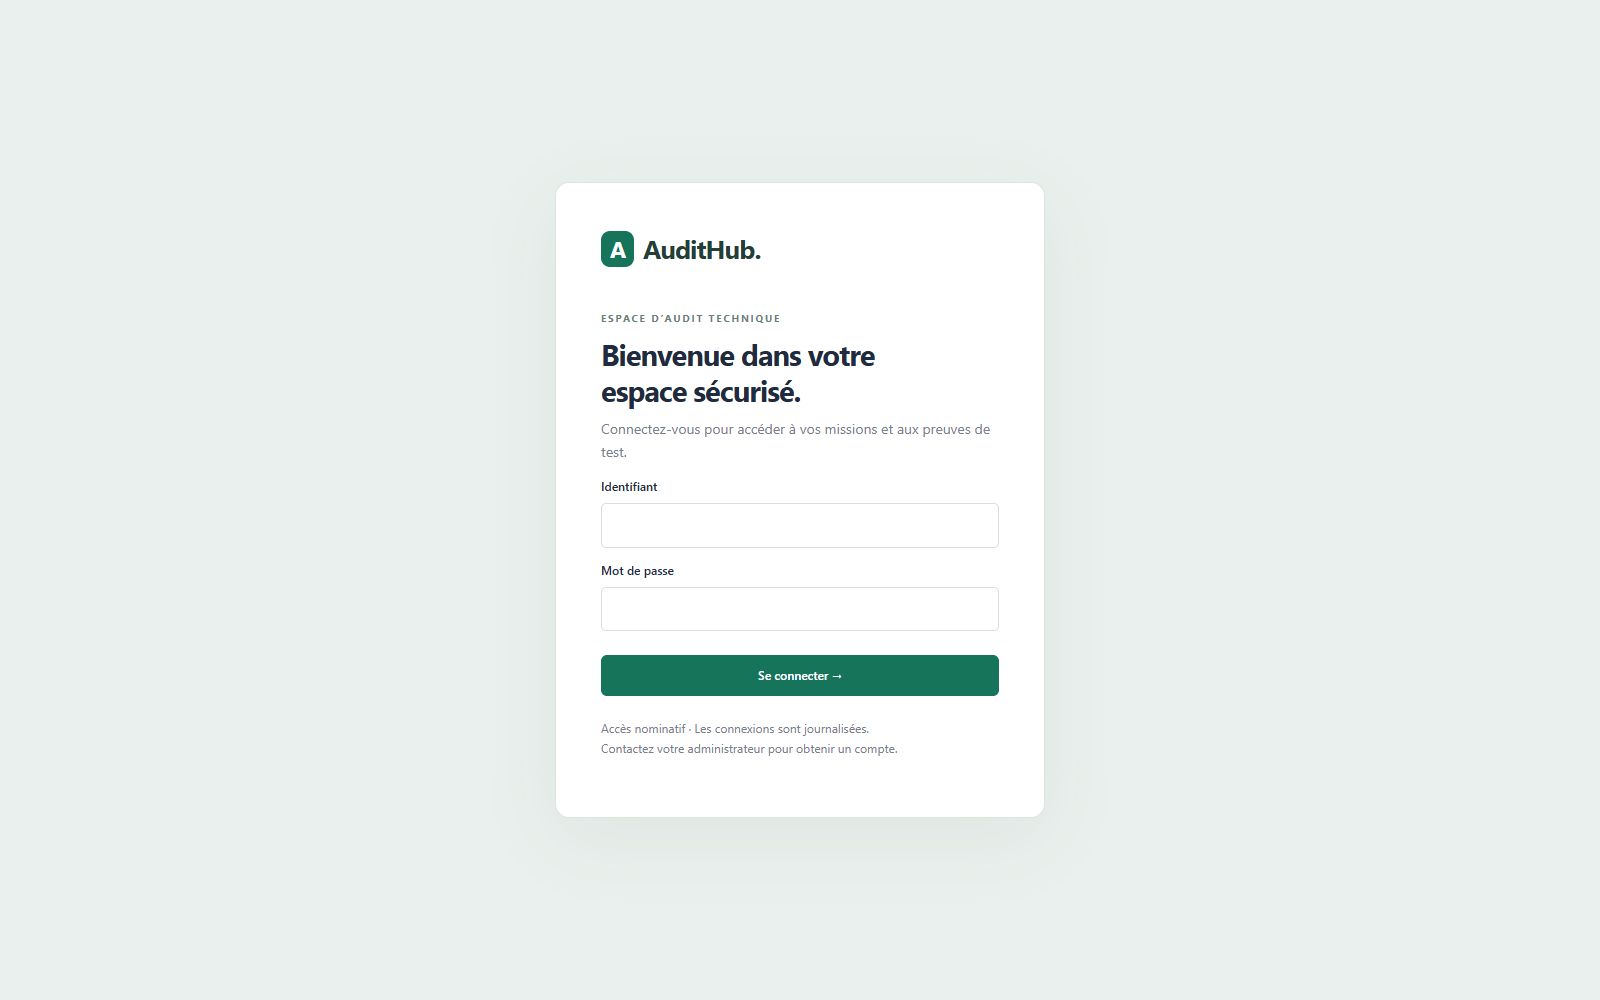
\includegraphics[width=.82\textwidth]{figures/screenshots/01-connexion.png}
\caption{Page de connexion r\'eelle d'AuditHub}
\label{fig:login}
\end{figure}

\begin{figure}[H]
\centering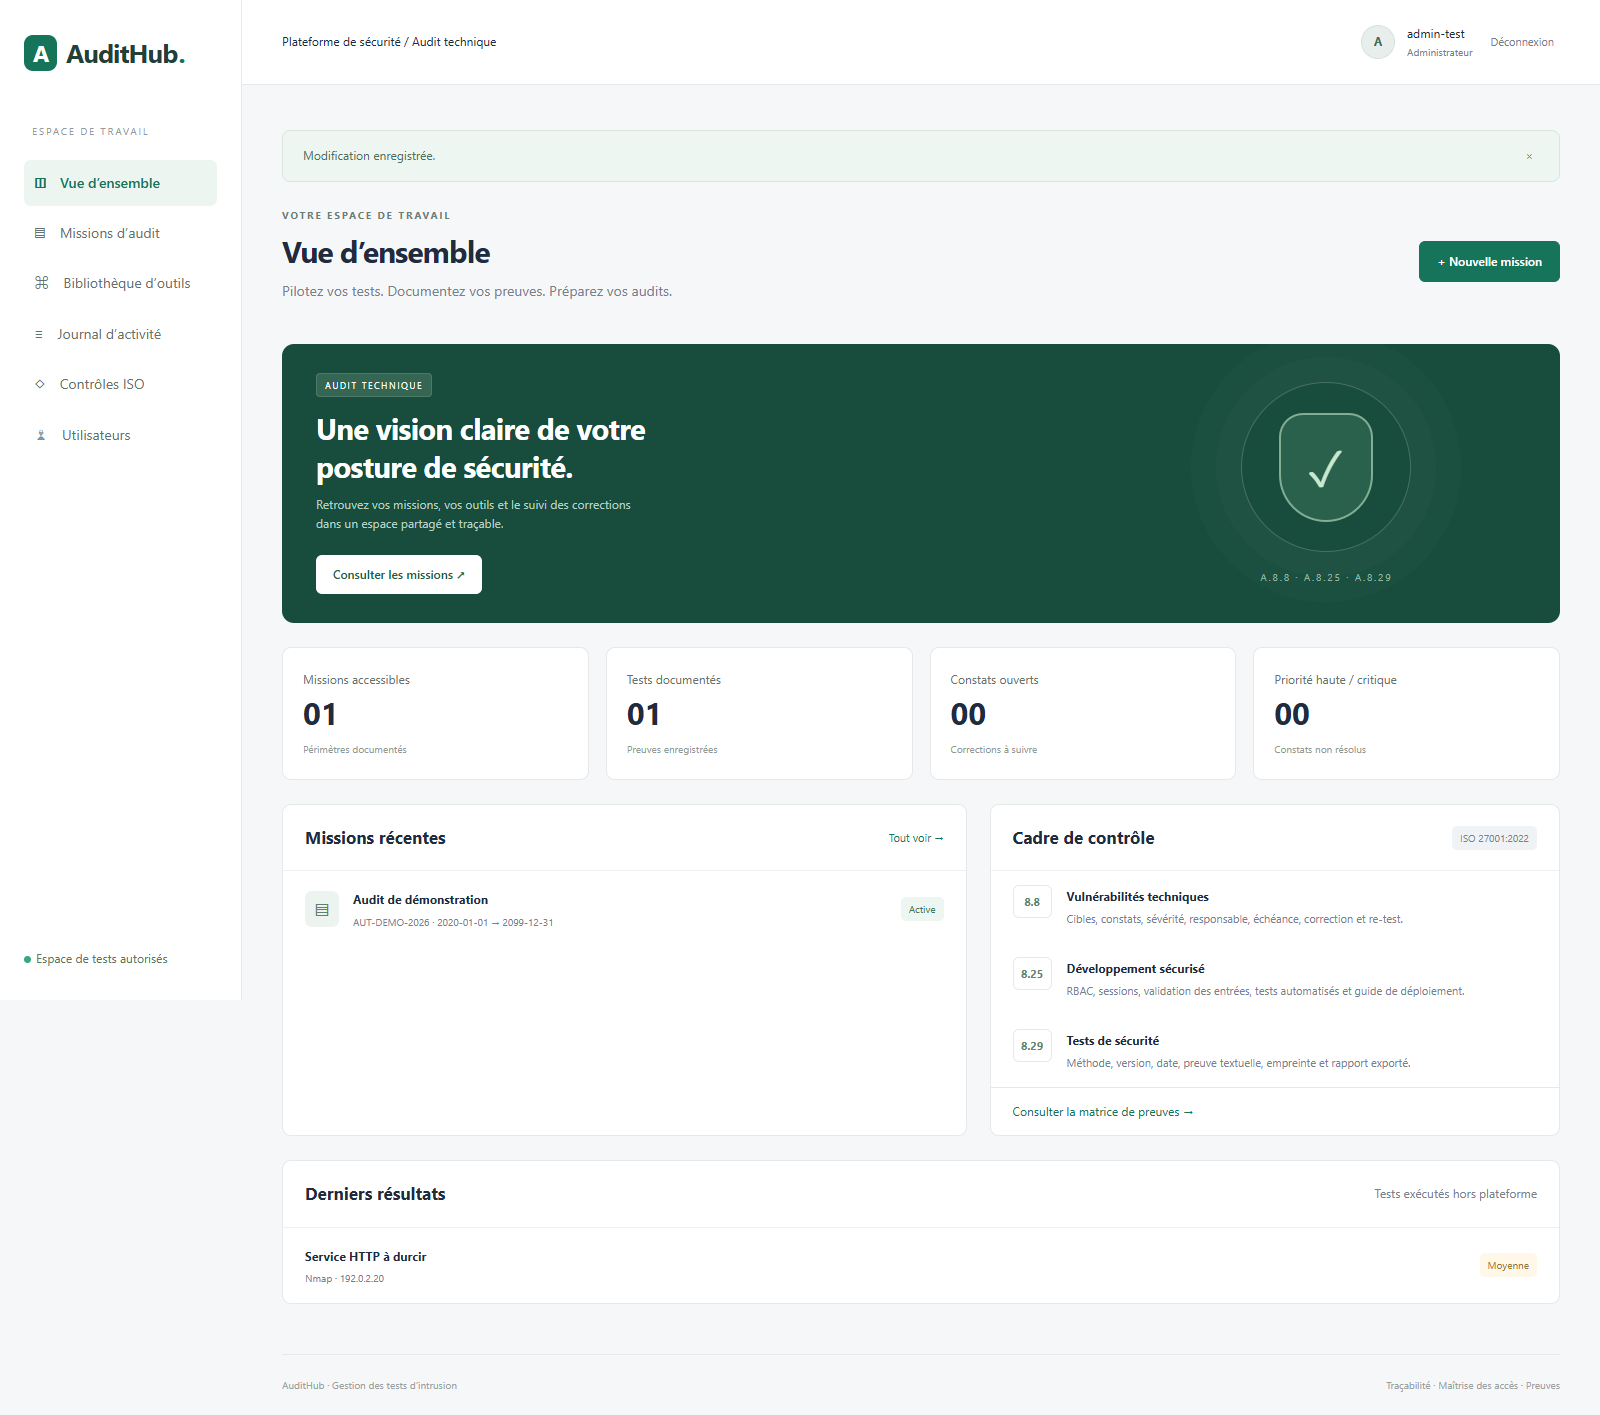
\includegraphics[width=.98\textwidth]{figures/screenshots/06-tableau-de-bord.png}
\caption{Tableau de bord aliment\'e par des donn\'ees synth\'etiques}
\label{fig:dashboard}
\end{figure}

\section*{D\'emonstration du flux d'audit}
\addcontentsline{toc}{section}{D\'emonstration du flux d'audit}
La campagne de capture cr\'ee une mission \og Audit de d\'emonstration \fg{} dans une base temporaire, lui associe un p\'erim\`etre IPv4/IPv6, consigne un constat Nmap, puis enregistre un re-test. Les informations sont synth\'etiques et n'exposent aucune donn\'ee de la base de travail.

\begin{figure}[H]
\centering
\begin{subfigure}{.48\textwidth}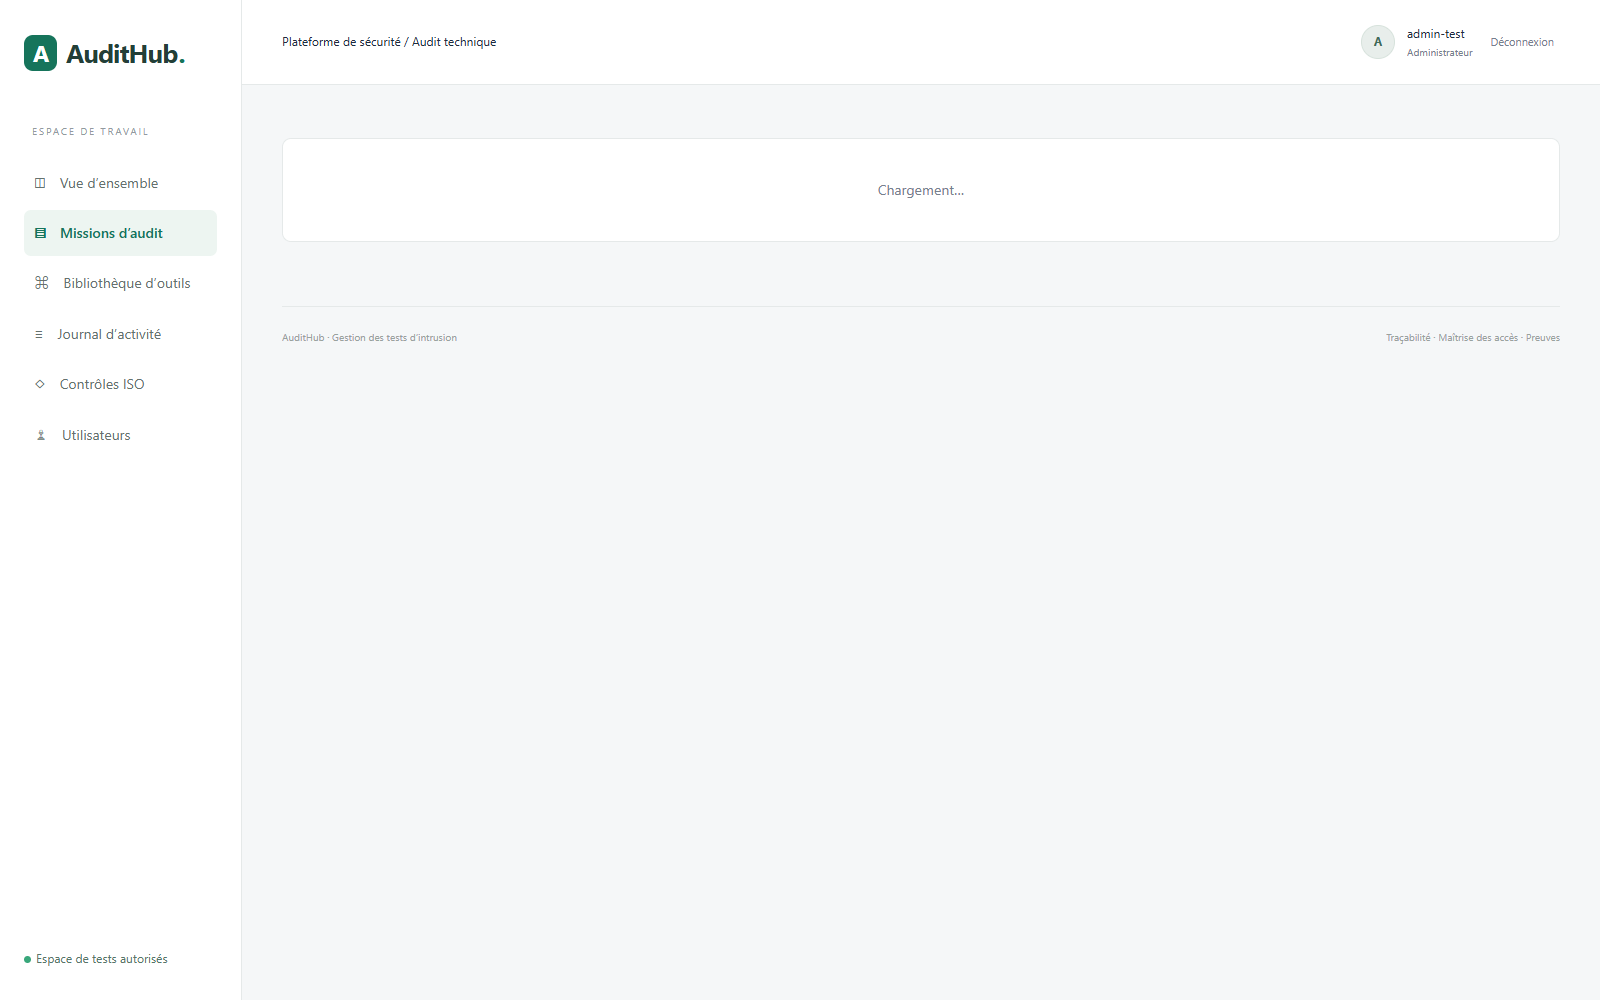
\includegraphics[width=\linewidth]{figures/screenshots/02-creation-mission.png}\caption{Formulaire de mission}\end{subfigure}\hfill
\begin{subfigure}{.48\textwidth}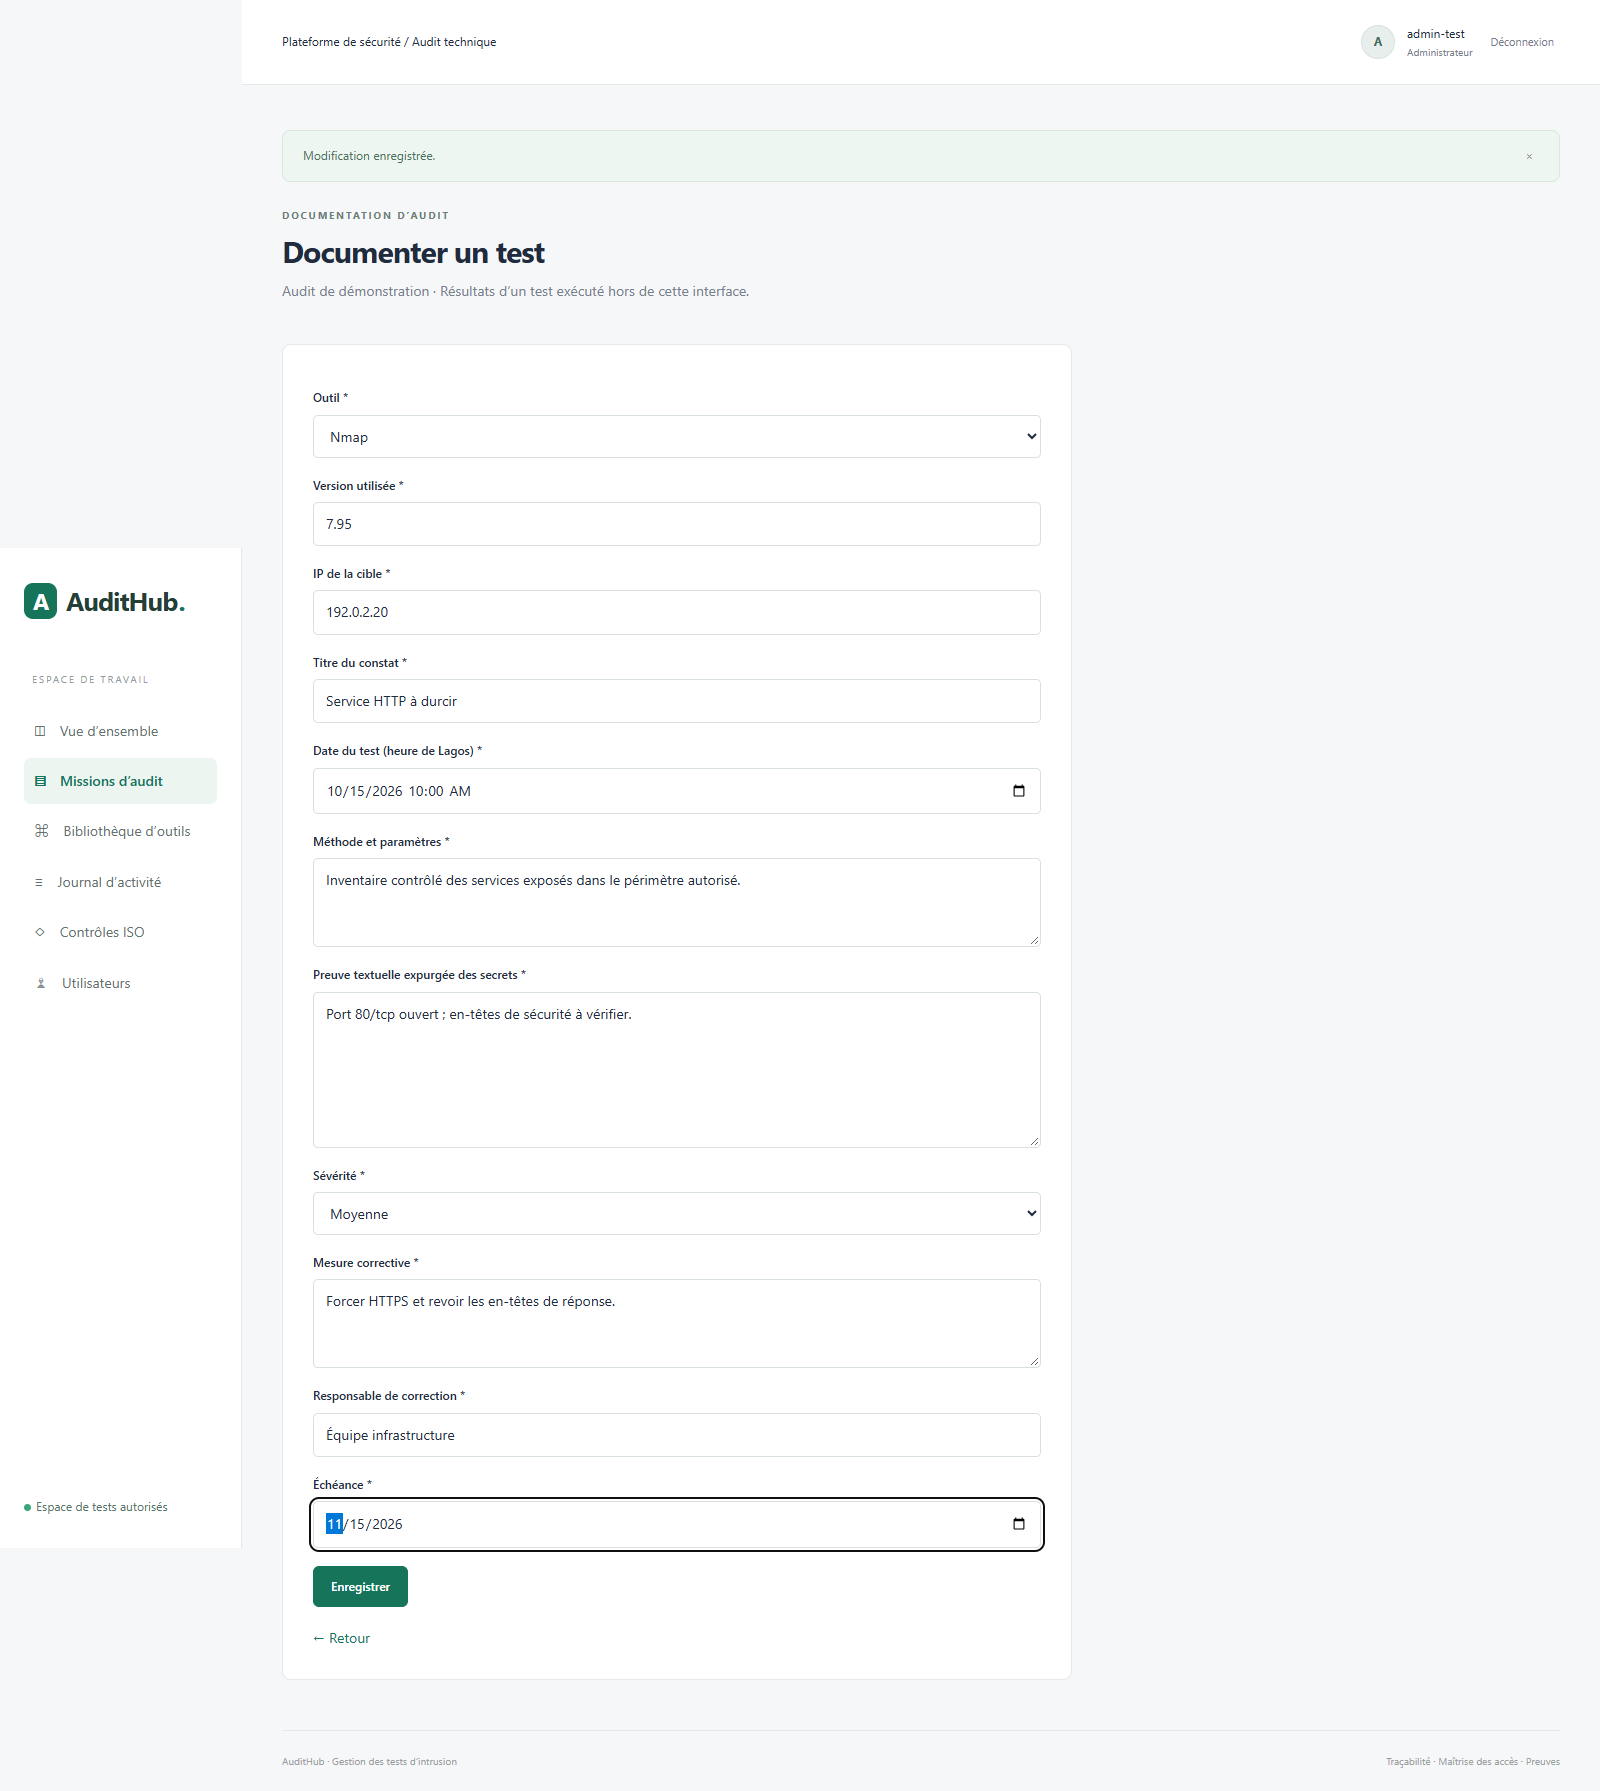
\includegraphics[width=\linewidth]{figures/screenshots/03-saisie-resultat.png}\caption{Saisie d'un r\'esultat}\end{subfigure}
\caption{Cr\'eation du p\'erim\`etre et documentation d'un test}
\label{fig:forms}
\end{figure}

\begin{figure}[H]
\centering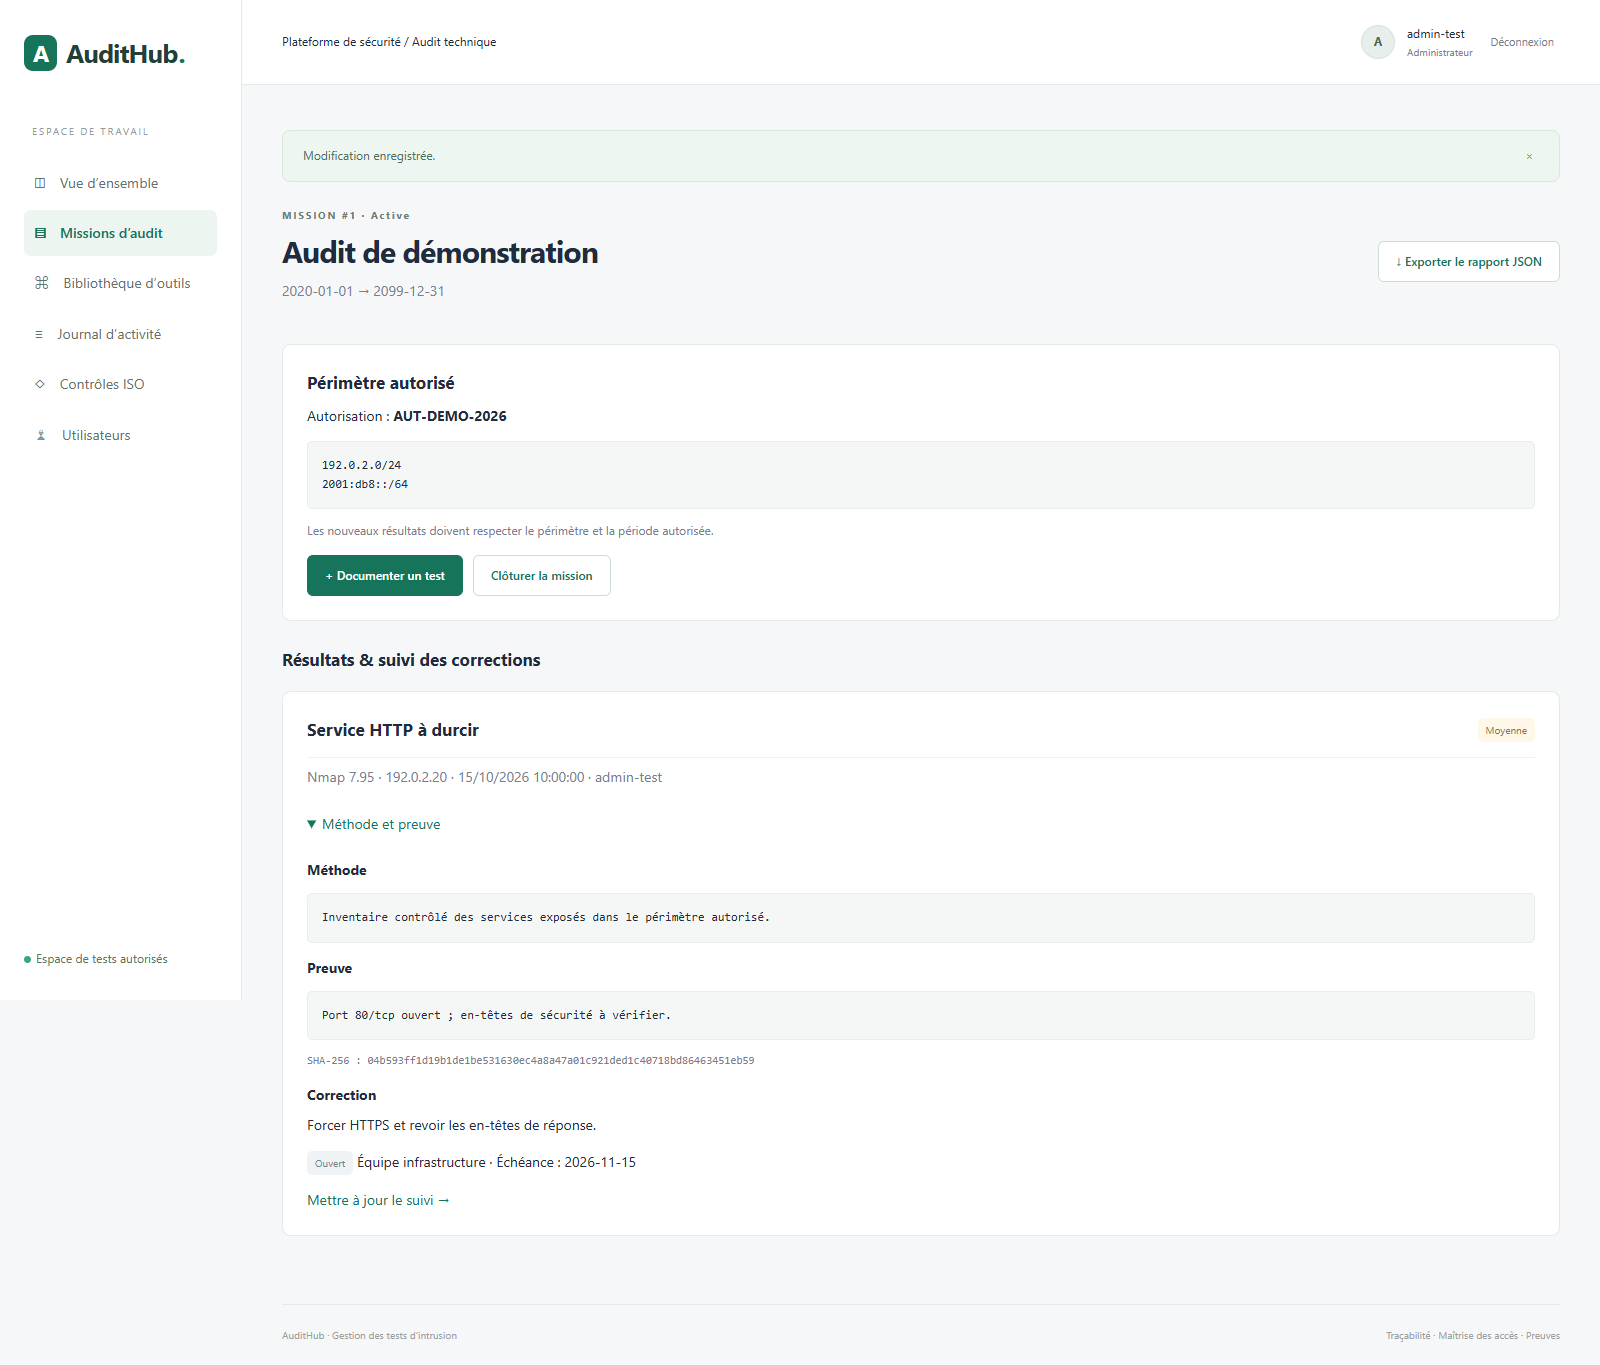
\includegraphics[width=.96\textwidth]{figures/screenshots/04-detail-mission.png}
\caption{D\'etail d'une mission avec preuve textuelle et empreinte SHA-256}
\label{fig:mission-detail}
\end{figure}

\begin{figure}[H]
\centering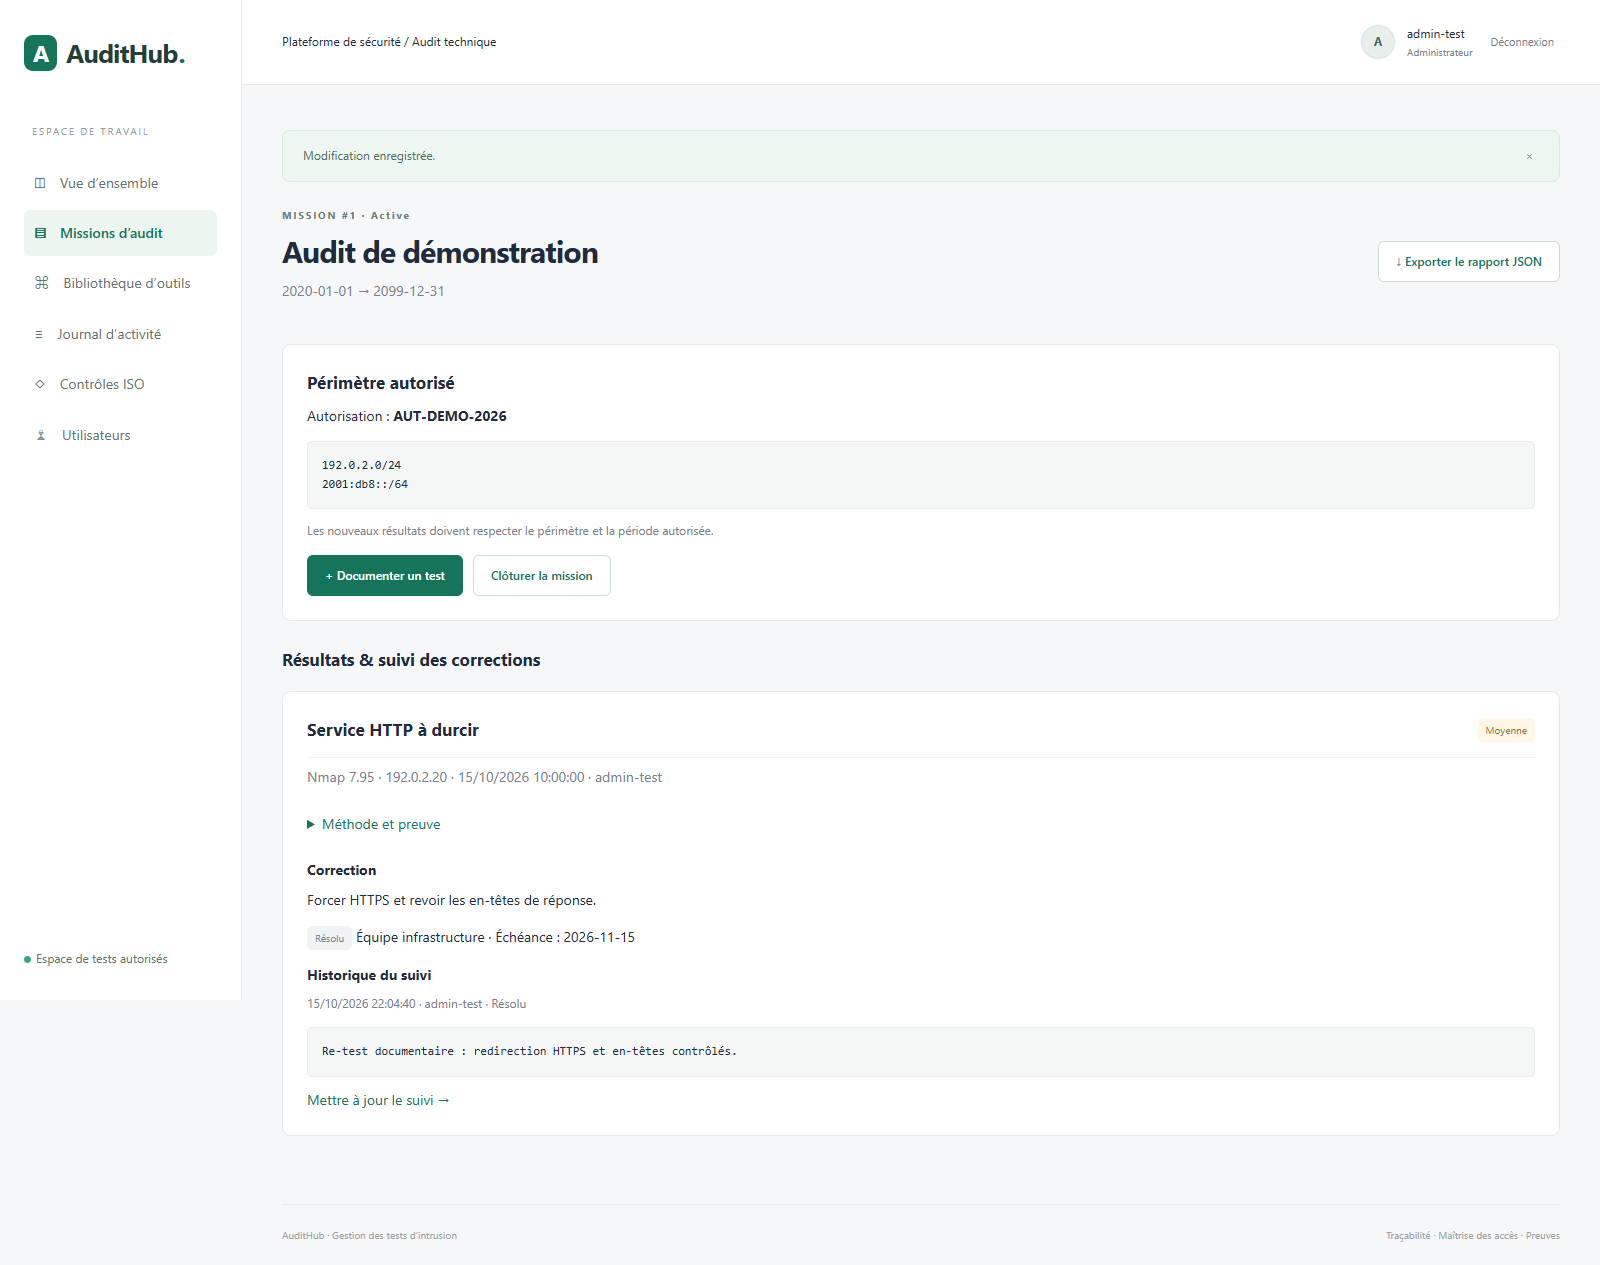
\includegraphics[width=.96\textwidth]{figures/screenshots/05-historique-suivi.png}
\caption{Historique dat\'e d'un suivi de correction}
\label{fig:followup}
\end{figure}

\section*{S\'ecurit\'e impl\'ement\'ee}
\addcontentsline{toc}{section}{S\'ecurit\'e impl\'ement\'ee}
\begin{itemize}
  \item mot de passe hach\'e par Django et validateurs imposant notamment 12 caract\`eres ;
  \item session de 30 minutes d'inactivit\'e, expiration \`a la fermeture, cookie HttpOnly et SameSite Strict ;
  \item cookies Secure, redirection HTTPS et HSTS hors mode d\'eveloppement ;
  \item jeton CSRF renouvel\'e apr\`es connexion et mutations POST ;
  \item CSP sans script inline/eval, refus du framing, politique de permissions restrictive et \evidence{no-store} ;
  \item limitation par compte (5 \`echecs) et par IP (30 \`echecs) sur 15 minutes ; les succ\`es ne consomment pas le quota ;
  \item filtrage des missions avant lecture, \`ecriture et export ;
  \item preuve initiale non modifiable dans l'interface et empreinte SHA-256 ;
  \item journalisation des actions sensibles et historique des suivis.
\end{itemize}
Ces mesures ne garantissent pas l'inviolabilit\'e face \`a un administrateur de base. L'empreinte stock\'ee avec la preuve n'est pas une signature externe.

\begin{figure}[H]
\centering
\begin{subfigure}{.48\textwidth}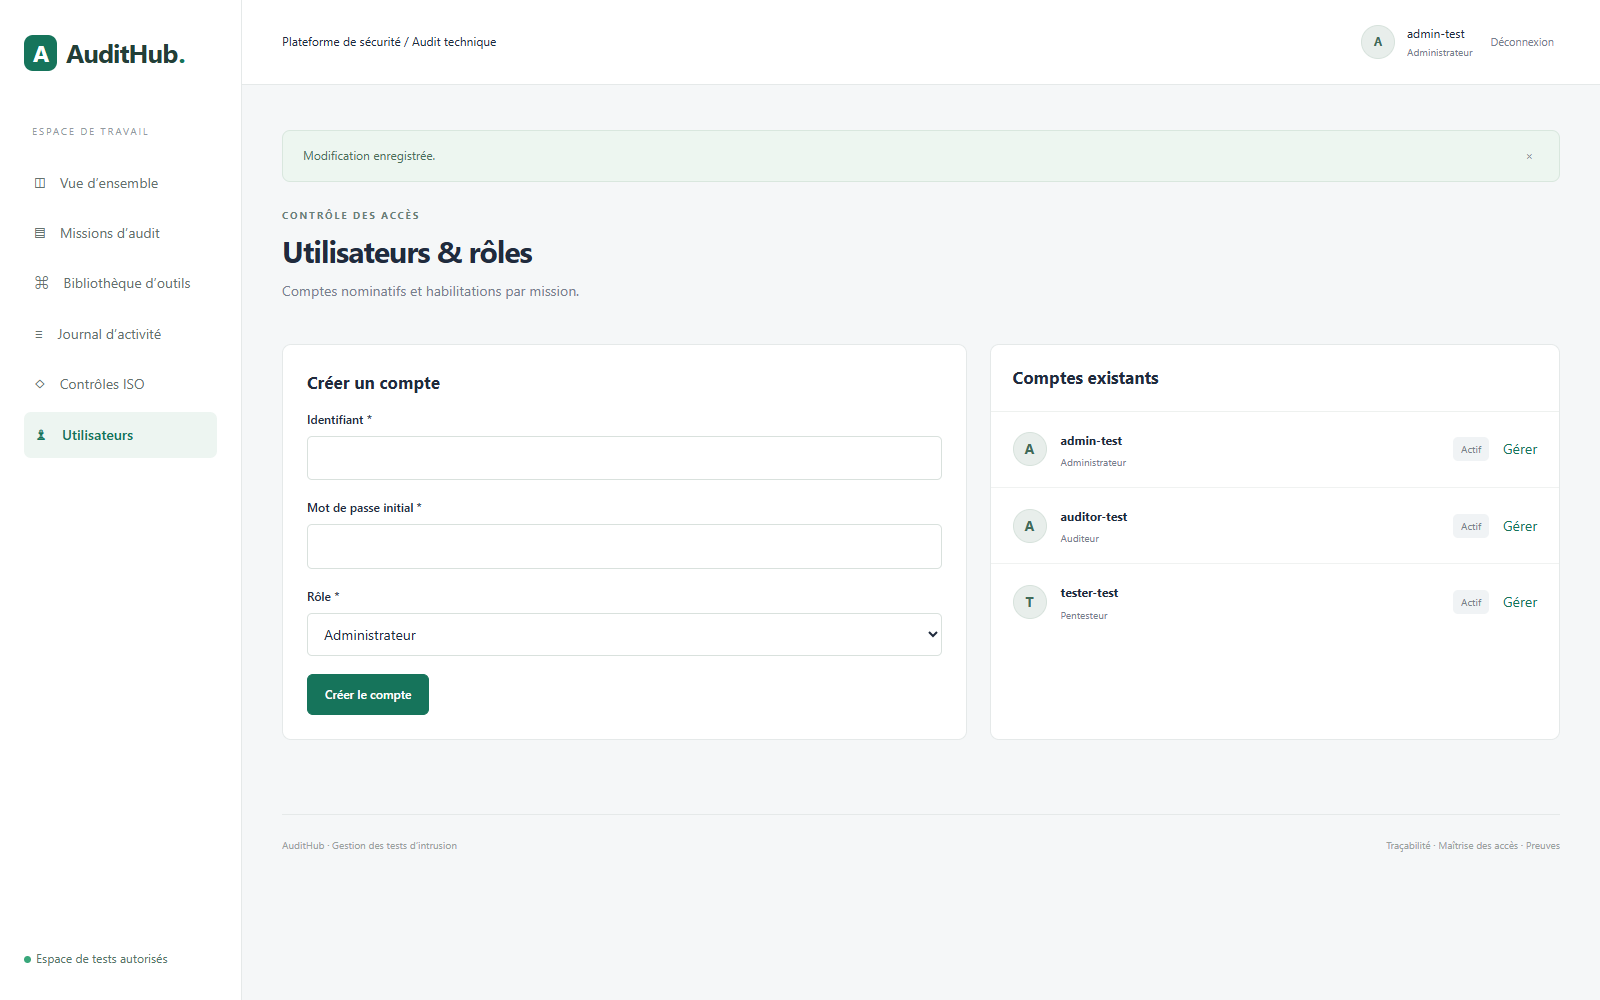
\includegraphics[width=\linewidth]{figures/screenshots/07-utilisateurs-roles.png}\caption{Comptes et r\^oles}\end{subfigure}\hfill
\begin{subfigure}{.48\textwidth}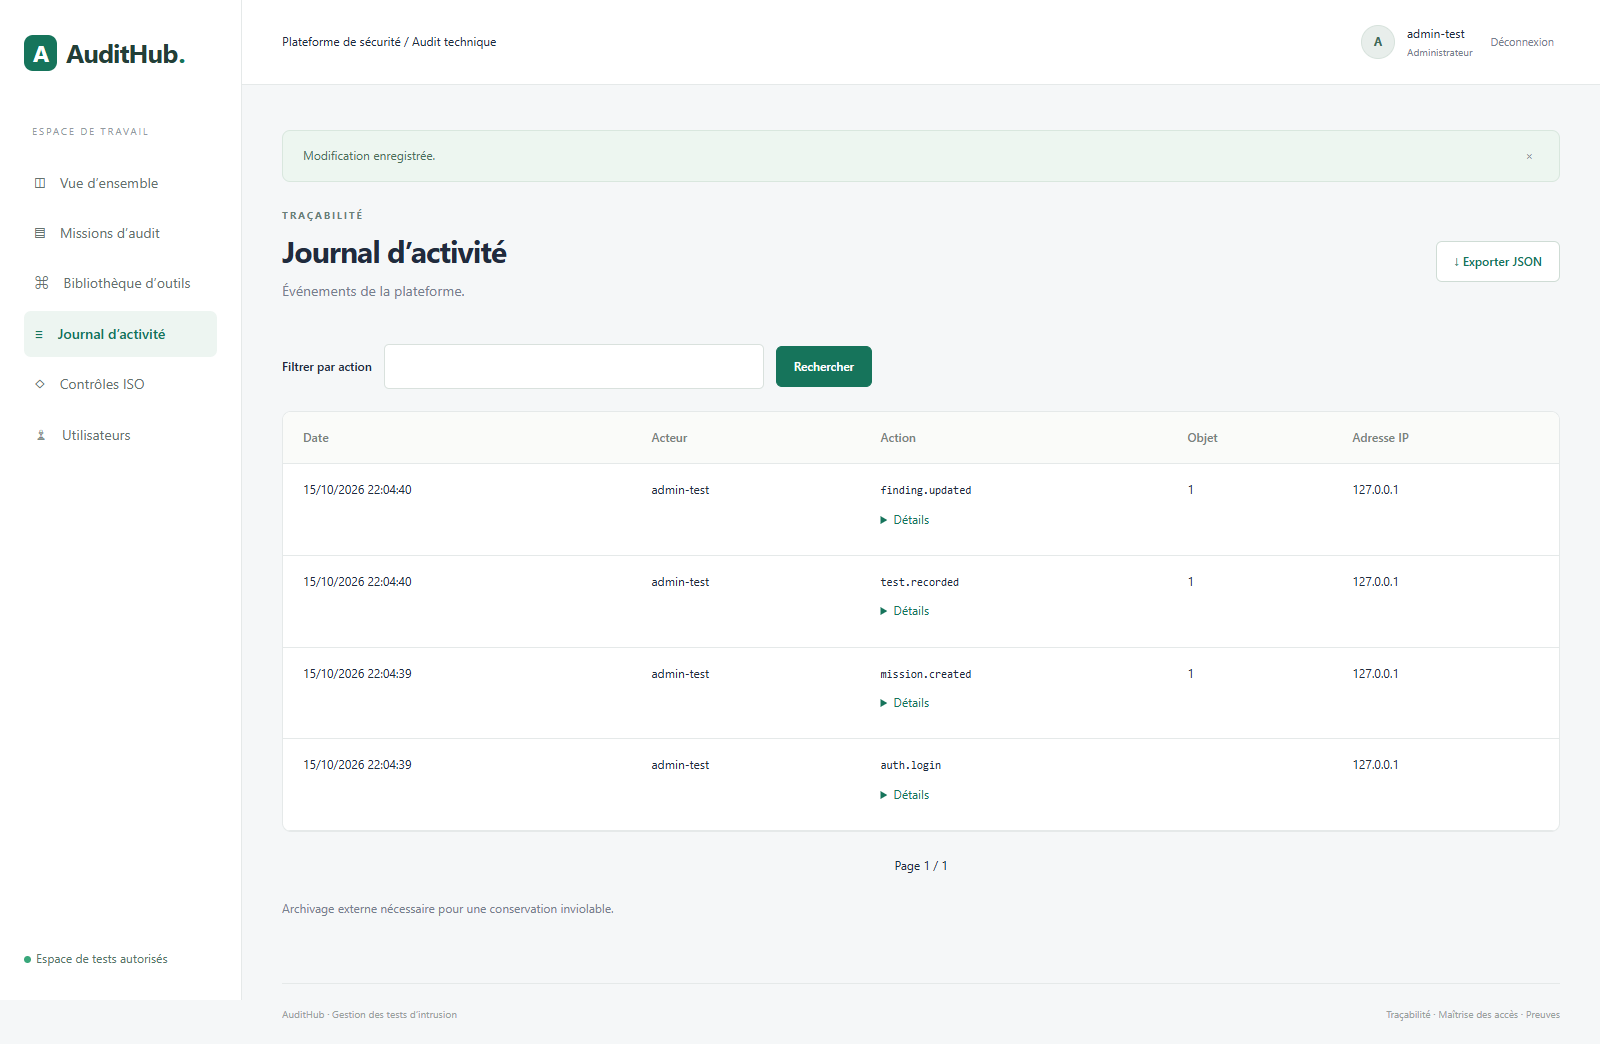
\includegraphics[width=\linewidth]{figures/screenshots/08-journal.png}\caption{Journal d'activit\'e}\end{subfigure}
\caption{Fonctions d'administration et de tra\c{c}abilit\'e}
\label{fig:admin-log}
\end{figure}

\chapter{SYNTH\`ESE DES CONSTATATIONS}

\section*{8.1 Statistiques globales}
\addcontentsline{toc}{section}{8.1 Statistiques globales}
La notion de non-conformit\'e de certification n'est pas applicable faute d'audit organisationnel. La synth\`ese ci-dessous porte sur le logiciel et distingue les capacit\'es valid\'ees des limites connues.

\begin{table}[H]
\centering
\caption{Indicateurs objectifs de la version finale}
\begin{tabularx}{\textwidth}{X r l}
\toprule
\rowcolor{AuditLight}Indicateur & Valeur & Source\\
\midrule
Tests backend ex\'ecut\'es & 33/33 & \evidence{manage.py test}\\
Parcours navigateur ex\'ecut\'es & 3/3 & Playwright, Chrome headless\\
Captures de rapport & 9 & sc\'enario isol\'e\\
R\^oles applicatifs & 3 & \evidence{portal.security.ROLES}\\
Outils document\'es & 4 & Nmap, Metasploit, Burp Suite, ZAP\\
Migrations applicatives & 2 & \evidence{portal/migrations}\\
Erreurs de check Django & 0 & modes d\'eveloppement et production\\
Migrations manquantes & 0 & \evidence{makemigrations --check}\\
\bottomrule
\end{tabularx}
\end{table}

\section*{8.2 R\'epartition par article / mesure}
\addcontentsline{toc}{section}{8.2 R\'epartition par article / mesure}
\begin{longtable}{p{2.4cm}p{5.4cm}p{7cm}}
\caption{Contribution technique aux mesures cibl\'ees}\\
\toprule
\rowcolor{AuditLight}Mesure & Contribution d'AuditHub & Compl\'ements organisationnels n\'ecessaires\\
\midrule\endfirsthead
\toprule Mesure & Contribution & Compl\'ements requis\\\midrule\endhead
A.8.8 & registre de constats, cible, s\'ev\'erit\'e, responsable, \`ech\'eance, correction et re-test & inventaire d'actifs complet, veille, SLA, acceptation des risques, exceptions\\
A.8.25 & RBAC, validation, sessions, tests automatis\'es, CI et guide de d\'eploiement & politique de d\'eveloppement, revues ind\'ependantes, SAST/SCA, s\'eparation des environnements\\
A.8.29 & m\'ethode, outil/version, date, preuve, empreinte et historique de re-test & plan de recette sign\'e, crit\`eres de sortie, environnement cible et validation ind\'ependante\\
\bottomrule
\end{longtable}

\begin{figure}[H]
\centering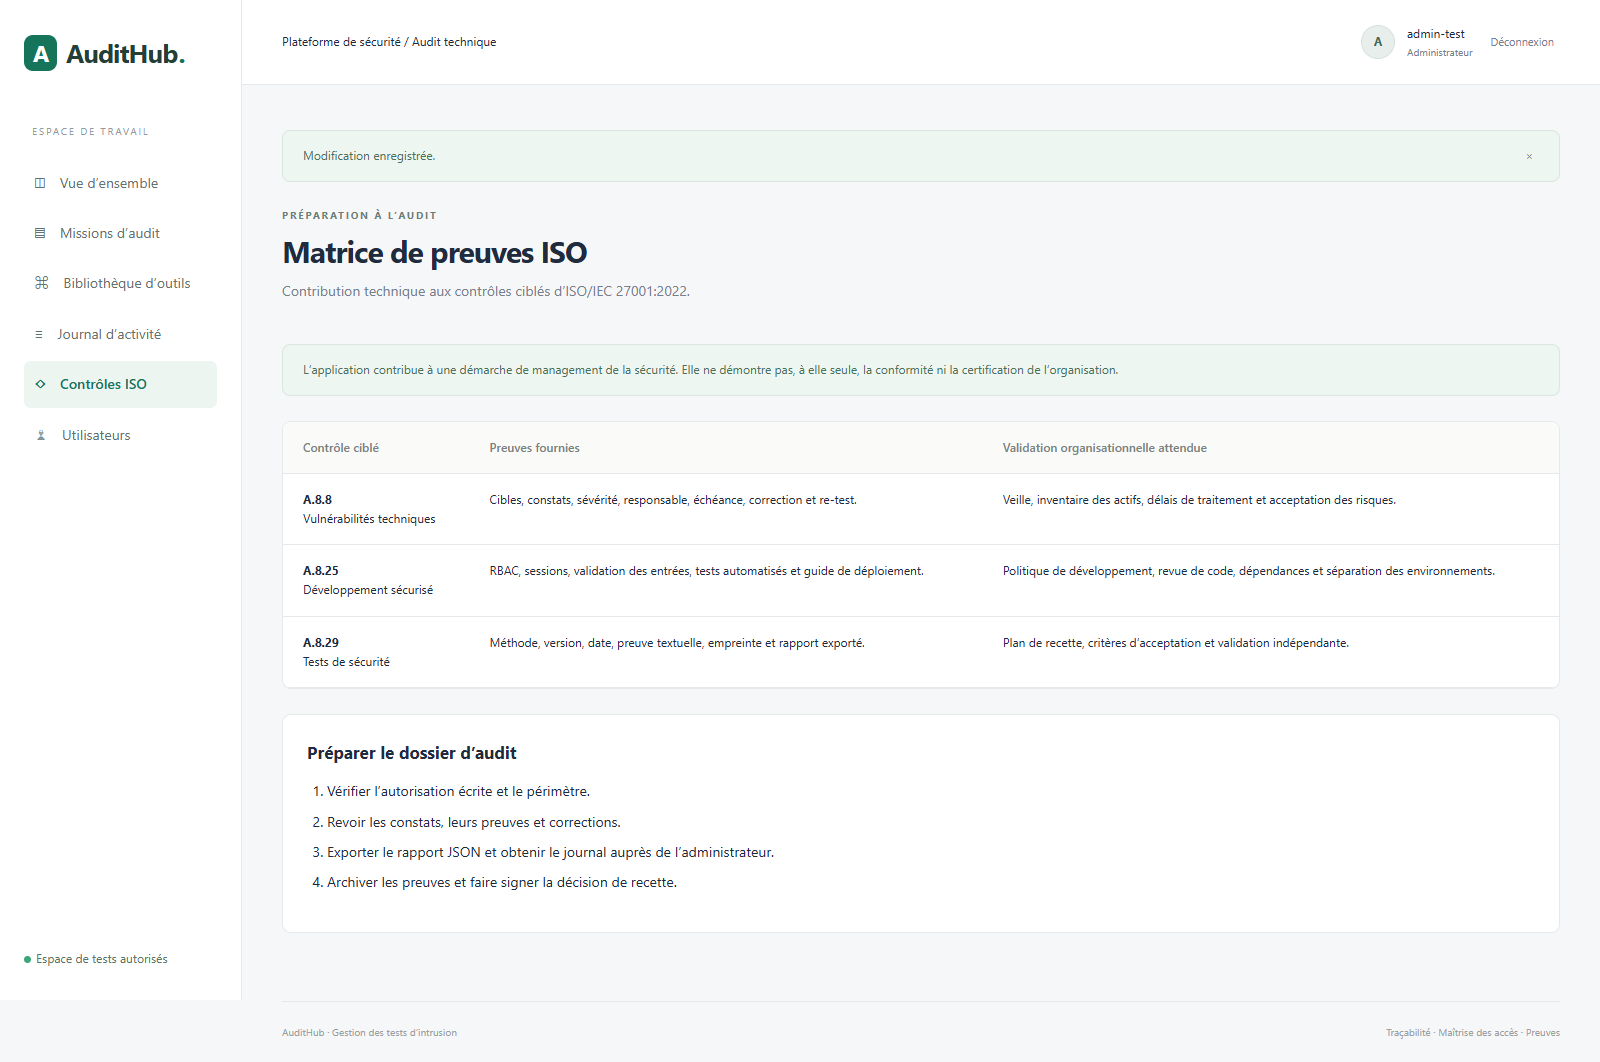
\includegraphics[width=.95\textwidth]{figures/screenshots/09-controles-iso.png}
\caption{Matrice ISO affich\'ee par l'application, explicitement pr\'esent\'ee comme contribution}
\label{fig:iso}
\end{figure}

\section*{Points forts identifi\'es}
\addcontentsline{toc}{section}{Points forts identifi\'es}
\begin{itemize}
  \item s\'eparation nette entre ex\'ecution offensive et gestion documentaire ;
  \item permissions serveur compl\'et\'ees par un cloisonnement au niveau des requ\^etes ;
  \item parcours de preuve coh\'erent, de l'autorisation \`a l'historique de correction ;
  \item gestion explicite des erreurs JSON et des erreurs de formulaires ;
  \item interface responsive sans ressource CDN et bundle reproductible via \evidence{npm ci} ;
  \item tests de s\'ecurit\'e ciblant CSRF, XSS, RBAC, p\'erim\`etre, dates, hachage et throttling ;
  \item documentation honn\^ete sur les limites et absence de revendication de certification.
\end{itemize}

\chapter{NON-CONFORMIT\'ES D\'ETAILL\'EES}

\section*{Position de la revue}
\addcontentsline{toc}{section}{Position de la revue}
Aucune non-conformit\'e ISO/IEC 27001 formelle n'est prononc\'ee. Une telle qualification exigerait un organisme audit\'e, un p\'erim\`etre SMSI, des crit\`eres contractuels, des preuves organisationnelles et une autorit\'e d'audit. La pr\'esente section recense plut\^ot les \textbf{\'ecarts techniques et limites de mise en production} objectivement observables.

\section*{\'Ecart technique ET-01 --- persistance mono-instance}
\addcontentsline{toc}{section}{ET-01 --- persistance mono-instance}
\begin{tabularx}{\textwidth}{>{\bfseries}p{3.8cm}X}
\toprule
Crit\`ere & Exploitation fiable en contexte multi-utilisateur\\
Constat & La configuration utilise un fichier SQLite local avec un d\'elai d'attente de 20 secondes.\\
Risque & Contention en \`ecriture, absence de haute disponibilit\'e et sauvegarde d\'ependante du syst\`eme de fichiers.\\
Preuve & \evidence{config/settings.py}, variable \evidence{DATABASES}.\\
Recommandation & Valider la concurrence attendue puis rendre la base configurable et migrer vers PostgreSQL si la charge ou la criticit\'e l'exigent.\\
\bottomrule
\end{tabularx}

\section*{\'Ecart technique ET-02 --- journal non inviolable}
\addcontentsline{toc}{section}{ET-02 --- journal non inviolable}
\begin{tabularx}{\textwidth}{>{\bfseries}p{3.8cm}X}
\toprule
Crit\`ere & Conservation ind\'ependante des traces\\
Constat & Les \evidence{AuditEvent} sont stock\'es dans la m\^eme base que les donn\'ees m\'etier. Aucun endpoint ne les modifie, mais un administrateur syst\`eme ou de base peut les alt\'erer.\\
Risque & Perte ou modification de la preuve de tra\c{c}abilit\'e.\\
Recommandation & Exporter vers un stockage externe \`a r\'etention contr\^ol\'ee et superviser les ruptures de collecte.\\
\bottomrule
\end{tabularx}

\section*{\'Ecart technique ET-03 --- identit\'e et r\'ecup\'eration de compte}
\addcontentsline{toc}{section}{ET-03 --- identit\'e et r\'ecup\'eration de compte}
\begin{tabularx}{\textwidth}{>{\bfseries}p{3.8cm}X}
\toprule
Crit\`ere & Cycle de vie complet de l'identit\'e\\
Constat & Les r\^oles et l'activation sont administrables et journalis\'es. Le changement de mot de passe reste une commande locale ; il n'existe ni r\'ecup\'eration autonome, ni MFA, ni SSO.\\
Risque & D\'ependance \`a l'administrateur syst\`eme et protection d'identit\'e limit\'ee pour un contexte sensible.\\
Recommandation & Choisir un fournisseur d'identit\'e selon le contexte, imposer MFA et d\'efinir un parcours de r\'ecup\'eration audit\'e.\\
\bottomrule
\end{tabularx}

\section*{\'Ecart technique ET-04 --- preuves uniquement textuelles}
\addcontentsline{toc}{section}{ET-04 --- preuves uniquement textuelles}
\begin{tabularx}{\textwidth}{>{\bfseries}p{3.8cm}X}
\toprule
Crit\`ere & Conservation compl\`ete des r\'esultats techniques\\
Constat & La preuve est un texte limit\'e \`a 20 000 caract\`eres. L'application ne re\c{c}oit pas les rapports natifs, captures ou pi\`eces jointes.\\
Risque & D\'etails techniques incomplets et d\'ependance \`a un r\'ef\'erentiel externe pour les originaux.\\
Recommandation & Si le besoin est valid\'e, ajouter un stockage de fichiers isol\'e, antivirus, quotas, empreintes externes, contr\^oles d'acc\`es et r\'etention.\\
\bottomrule
\end{tabularx}

\section*{\'Ecart technique ET-05 --- assurance de livraison partielle}
\addcontentsline{toc}{section}{ET-05 --- assurance de livraison partielle}
\begin{tabularx}{\textwidth}{>{\bfseries}p{3.8cm}X}
\toprule
Crit\`ere & Cha\^ine de livraison s\'ecuris\'ee\\
Constat & Une CI ex\'ecute build et tests ; les versions Python et npm sont verrouill\'ees. Aucun SBOM, SAST/SCA, signature d'artefact ou scan DAST n'est fourni.\\
Risque & Vuln\'erabilit\'es de d\'ependances ou d'impl\'ementation non d\'etect\'ees automatiquement.\\
Recommandation & Ajouter analyse de d\'ependances, SAST, SBOM, contr\^ole des secrets et signature des livrables.\\
\bottomrule
\end{tabularx}

\section*{\'Ecart technique ET-06 --- exploitation \`a finaliser}
\addcontentsline{toc}{section}{ET-06 --- exploitation \`a finaliser}
Le d\'ep\^ot documente Waitress et le proxy, mais ne fournit pas le proxy TLS, les certificats, un service syst\`eme, une supervision, des alertes ni une preuve de restauration. Ces \`el\'ements d\'ependent de l'environnement cible et doivent \^etre valid\'es avant exposition r\'eseau.

\begin{table}[H]
\centering
\caption{Priorisation propos\'ee des limites}
\begin{tabularx}{\textwidth}{p{2cm}X p{2.6cm}p{2.6cm}}
\toprule
\rowcolor{AuditLight}ID & Limite & Priorit\'e & Horizon\\
\midrule
ET-01 & base et concurrence & Haute si production partag\'ee & avant production\\
ET-02 & journal externe & Haute pour valeur probatoire & avant production\\
ET-03 & MFA/SSO/r\'ecup\'eration & Moyenne \`a haute & selon risques\\
ET-04 & pi\`eces jointes & Moyenne & selon besoin\\
ET-05 & assurance CI & Moyenne & prochaine it\'eration\\
ET-06 & exploitation & Haute & avant production\\
\bottomrule
\end{tabularx}
\end{table}

\chapter{OBSERVATIONS ET OPPORTUNIT\'ES D'AM\'ELIORATION}

\section*{Observation O-01 --- coh\'erence documentaire}
\addcontentsline{toc}{section}{O-01 --- coh\'erence documentaire}
La documentation expose clairement le mode documentaire et ses limites. Elle doit rester synchronis\'ee avec les nombres de tests, la version du sch\'ema d'export et les variables de proxy. La CI pourrait produire automatiquement un r\'esum\'e de validation afin de r\'eduire les informations dat\'ees.

\section*{Observation O-02 --- accessibilit\'e et navigateurs}
\addcontentsline{toc}{section}{O-02 --- accessibilit\'e et navigateurs}
Les formulaires utilisent labels, messages ARIA et \`etats de chargement. Le navigateur automatis\'e couvre Chrome et un affichage mobile, mais aucun audit WCAG outill\'e ni test Firefox/WebKit n'est pr\'esent. Une campagne axe-core et des tests clavier constitueraient une am\'elioration mesurable.

\section*{Observation O-03 --- score de risque}
\addcontentsline{toc}{section}{O-03 --- score de risque}
La s\'ev\'erit\'e est d\'eclarative. L'ajout d'un vecteur CVSS valid\'e, distinct de la priorit\'e m\'etier, permettrait de documenter le calcul sans remplacer le jugement de l'auditeur. Ce besoin n'est pas impl\'ement\'e dans la version analys\'ee.

\section*{Observation O-04 --- int\'egration d'outils}
\addcontentsline{toc}{section}{O-04 --- int\'egration d'outils}
Une extension d'ex\'ecution ne devrait pas \^etre ajout\'ee au serveur web. La documentation propose \`a juste titre un worker isol\'e, une file de t\^aches, des profils autoris\'es, des quotas, un arr\^et d'urgence et une validation du p\'erim\`etre juste avant l'ex\'ecution. Cette orientation est une opportunit\'e future et non une capacit\'e actuelle.

\section*{Bonne pratique BP-01 --- d\'efense en profondeur}
\addcontentsline{toc}{section}{BP-01 --- d\'efense en profondeur}
Les contr\^oles d'interface ne sont jamais la seule barri\`ere : permissions, filtrage des querysets, validation des formulaires, contraintes SQL, transactions et journalisation se compl\`etent. Cette combinaison facilite la maintenance et limite l'impact d'un contournement du frontend.

\section*{Bonne pratique BP-02 --- preuves reproductibles}
\addcontentsline{toc}{section}{BP-02 --- preuves reproductibles}
Les captures de ce rapport sont reproductibles par le sc\'enario Playwright fourni. Celui-ci lance une base temporaire, cr\'ee trois comptes synth\'etiques, remplit une mission et s'arr\^ete sans toucher \`a \evidence{audit.sqlite3}. Cette approche garantit que les figures correspondent \`a l'application et non \`a des maquettes.

\chapter{CONCLUSION ET RECOMMANDATION DE CERTIFICATION}

\section*{11.1 Synth\`ese g\'en\'erale}
\addcontentsline{toc}{section}{11.1 Synth\`ese g\'en\'erale}
AuditHub atteint son objectif de \textbf{prototype fonctionnel de gestion documentaire d'audits techniques}. La cha\^ine mission--autorisation--p\'erim\`etre--constat--preuve--correction--re-test est coh\'erente, contr\^ol\'ee par r\^oles et couverte par des tests. L'architecture Django/React de m\^eme origine est simple \`a d\'eployer, et l'interface fournit des parcours utilisables sans serveur frontend distinct.

Les 33 tests Django et les 3 parcours navigateur r\'eussissent dans l'environnement de validation. Le build React aboutit, les migrations sont coh\'erentes et le check Django ne signale pas de probl\`eme avec une configuration de production valide. Ces r\'esultats prouvent les sc\'enarios couverts, pas l'absence g\'en\'erale de vuln\'erabilit\'es.

Le projet pr\'esente plusieurs qualit\'es d'ing\'enierie : validations c\^ot\'e serveur, RBAC, transactions, contraintes SQL, historique de suivi, configuration par environnement, d\'ependances verrouill\'ees, CI et documentation de d\'eploiement. Ses limites sont explicites : SQLite, absence de journal WORM, MFA/SSO, stockage de fichiers, surveillance et tests ind\'ependants.

\section*{Position relative \`a la certification}
\addcontentsline{toc}{section}{Position relative \`a la certification}
\textbf{Aucune recommandation de certification ISO/IEC 27001 n'est \`emise.} AuditHub fournit des \`el\'ements qui peuvent contribuer \`a A.8.8, A.8.25 et A.8.29, mais l'\'evaluation d'un SMSI suppose les articles 4 \`a 10, la D\'eclaration d'Applicabilit\'e, les risques, les politiques, les personnes, les processus et des preuves organisationnelles absentes de ce projet.

Dans un cadre acad\'emique, la version peut \^etre consid\'er\'ee comme \textbf{livrable logiciel valid\'e dans son p\'erim\`etre documentaire}, sous r\'eserve que l'\'evaluateur compl\`ete les informations institutionnelles et appr\'ecie les choix au regard du sujet initial non fourni dans le d\'ep\^ot.

\section*{11.4 Prochaines \`etapes}
\addcontentsline{toc}{section}{11.4 Prochaines \`etapes}
\begin{longtable}{p{5.4cm}p{4cm}p{5.3cm}}
\caption{Feuille de route recommand\'ee}\\
\toprule
\rowcolor{AuditLight}\`Etape & Responsable attendu & Condition de cl\^oture\\
\midrule\endfirsthead
\toprule \`Etape & Responsable & Condition\\\midrule\endhead
Compl\'eter auteur, encadrant et contexte acad\'emique & porteur du projet & informations confirm\'ees\\
Qualifier la charge et choisir la base & architecte / exploitation & essai de concurrence et sauvegarde\\
D\'eployer TLS, service et supervision & exploitation & recette de production document\'ee\\
Externaliser et prot\'eger les journaux & s\'ecurit\'e / exploitation & r\'etention et restauration test\'ees\\
Ajouter SAST/SCA/SBOM & \`equipe de d\'eveloppement & pipeline bloquant et rapports archiv\'es\\
Choisir MFA/SSO & responsable s\'ecurit\'e & authentification forte test\'ee\\
R\'ealiser une revue ind\'ependante & auditeur autoris\'e & rapport et actions suivies\\
\bottomrule
\end{longtable}

\chapter{ANNEXES}

\section*{Annexe A : Liste des documents examin\'es}
\addcontentsline{toc}{section}{Annexe A : Liste des documents examin\'es}
\begin{longtable}{r p{6cm} p{7cm}}
\toprule
\rowcolor{AuditLight}N\textsuperscript{o} & Document & Usage\\
\midrule\endfirsthead
\toprule N\textsuperscript{o} & Document & Usage\\\midrule\endhead
1 & \evidence{README.md} & fonctions, installation, validation et limites\\
2 & \evidence{docs/ARCHITECTURE.md} & architecture, menaces et d\'eploiement\\
3 & \evidence{docs/GUIDE\_AUDITEUR.md} & r\^oles et processus op\'erationnels\\
4 & \evidence{docs/RAPPORT\_TESTS\_ISO.md} & r\'esultats de validation et matrice ISO\\
5 & \evidence{Structure rapport.docx} & structure obligatoire et consignes de couleur\\
6 & \evidence{requirements*.txt}, \evidence{package*.json} & d\'ependances et versions\\
7 & \evidence{.github/workflows/ci.yml} & automatisation de validation\\
\bottomrule
\end{longtable}

\section*{Annexe B : Inventaire du code examin\'e}
\addcontentsline{toc}{section}{Annexe B : Inventaire du code examin\'e}
\begin{longtable}{p{5cm}p{9.5cm}}
\toprule
\rowcolor{AuditLight}Fichier / zone & Responsabilit\'e\\
\midrule\endfirsthead
\toprule Fichier / zone & Responsabilit\'e\\\midrule\endhead
\evidence{portal/models.py} & entit\'es, relations et contraintes\\
\evidence{portal/forms.py} & validation m\'etier et comptes\\
\evidence{portal/views.py} & cas d'usage, transactions, exports\\
\evidence{portal/security.py} & r\^oles, journal, IP client et en-t\^etes\\
\evidence{portal/api.py} & s\'erialisation JSON et erreurs\\
\evidence{config/settings.py} & sessions, HTTPS, cookies, base, limites\\
\evidence{config/urls.py} & surface HTTP et coque React\\
\evidence{frontend/src/main.jsx} & navigation et pages\\
\evidence{frontend/src/components.jsx} & composants, formulaires et constats\\
\evidence{frontend/src/api.js} & transport et erreurs\\
\evidence{portal/tests.py} & tests fonctionnels et de s\'ecurit\'e\\
\evidence{frontend/tests/workflows.spec.js} & tests bout en bout\\
\bottomrule
\end{longtable}

\section*{Annexe C : Matrice des permissions}
\addcontentsline{toc}{section}{Annexe C : Matrice des permissions}
\begin{table}[H]
\centering\small
\begin{tabularx}{\textwidth}{X c c c}
\toprule
\rowcolor{AuditLight}Action & Admin. & Pentesteur & Auditeur\\
\midrule
Consulter les outils & Oui & Oui & Oui\\
Cr\'eer une mission & Oui & Non & Non\\
Consulter/exporter une mission & Toutes & Affect\'ees & Affect\'ees\\
Documenter un test & Oui & Affect\'ees & Non\\
Suivre une correction & Oui & Affect\'ees & Non\\
Cl\^oturer/r\'eouvrir & Oui & Non & Non\\
Cr\'eer/g\'erer un compte & Oui & Non & Non\\
Journal global/export & Oui & Non & Non\\
Journal personnel & Oui & Non & Oui\\
\bottomrule
\end{tabularx}
\end{table}

\section*{Annexe D : Endpoints principaux}
\addcontentsline{toc}{section}{Annexe D : Endpoints principaux}
\begin{longtable}{p{5.3cm}p{2.2cm}p{6.7cm}}
\toprule
\rowcolor{AuditLight}Chemin API & M\'ethodes & Objet\\
\midrule\endfirsthead
\toprule Chemin & M\'ethodes & Objet\\\midrule\endhead
\evidence{/api/session/} & GET & profil, r\^ole et jeton CSRF\\
\evidence{/api/connexion/} & GET, POST & authentification et limitation\\
\evidence{/api/missions/} & GET & missions autoris\'ees, recherche et pagination\\
\evidence{/api/missions/nouvelle/} & GET, POST & cr\'eation administrateur\\
\evidence{/api/missions/<id>/} & GET & d\'etail et constats\\
\evidence{/api/missions/<id>/test/} & GET, POST & saisie de r\'esultat\\
\evidence{/api/tests/<id>/suivi/} & GET, POST & suivi et historique\\
\evidence{/api/missions/<id>/rapport/} & GET & export JSON v2\\
\evidence{/api/journal/} & GET & consultation autoris\'ee\\
\evidence{/api/journal/export/} & GET & export global administrateur\\
\evidence{/api/utilisateurs/} & GET, POST & comptes\\
\evidence{/api/utilisateurs/<id>/acces/} & GET, POST & r\^ole et activation\\
\bottomrule
\end{longtable}

\section*{Annexe E : Preuves documentaires collect\'ees}
\addcontentsline{toc}{section}{Annexe E : Preuves documentaires collect\'ees}
\begin{enumerate}
  \item sortie de 33 tests Django r\'eussis ;
  \item sortie de 3 parcours Playwright r\'eussis ;
  \item build esbuild termin\'e sans erreur ;
  \item checks Django en d\'eveloppement et production sans erreur ;
  \item v\'erification de migrations sans changement manquant ;
  \item neuf captures sous \evidence{figures/screenshots/} ;
  \item analyse de couleur du mod\`ele sous \evidence{template\_analysis.txt}.
\end{enumerate}

\section*{Annexe F : D\'eclaration de non-responsabilit\'e}
\addcontentsline{toc}{section}{Annexe F : D\'eclaration de non-responsabilit\'e}
Cette revue est fond\'ee sur l'\'etat disponible du d\'ep\^ot et sur des tests automatis\'es. Elle ne garantit pas l'absence de vuln\'erabilit\'e et ne remplace ni une recette de production, ni un test d'intrusion ind\'ependant, ni un audit de certification.

\section*{Annexe G : Confidentialit\'e}
\addcontentsline{toc}{section}{Annexe G : Confidentialit\'e}
Le rapport est destin\'e \`a l'\'evaluation acad\'emique. Les captures reposent sur des identifiants et donn\'ees synth\'etiques ; aucun mot de passe n'y appara\^it. Toute diffusion ult\'erieure doit respecter la politique de l'\'etablissement et les droits sur le code.

\section*{Signatures}
\addcontentsline{toc}{section}{Signatures}
\begin{tabularx}{\textwidth}{X X X}
\toprule
Auteur du projet & Professeur / encadrant & Date\\
\midrule
\vspace{1.8cm} & & 15/10/2026\\
\bottomrule
\end{tabularx}


\bibliographystyle{plain}
\bibliography{references}
\end{document}
